\textbf{Цель работы}: Получение навыков проведения исследований компьютерной математической модели, построенной на квазилинейном уравнении параболического типа.

Исследование проводится с помощью программы, созданной в лабораторной работе №4.

\section{ИСХОДНЫЕ ДАННЫЕ}

\begin{enumerate}
    \item Значения параметров (как в лабораторной работе №4)

        \begin{equation*}
            \begin{matrix*}[l]
                k(T) = a_1(b_1 + c_1 T^{m_1}), \frac{\text{Вт}}{\text{см К}}, \\
                c(T) = a_2 + b_2 T^{m_2} - \frac{c_2}{T^2}, \frac{\text{Дж}}{\text{см}^3 \text{К}}, \\
                a_1 = 0.0134,\ b_1 = 1,\ c_1 = 4.35 \cdot 10^{-4},\ m_1=1, \\
                a_2 = 2.049,\ b_2 = 0.563 \cdot 10^{-3},\ c_2 = 0.528 \cdot 10^5,\ m_2 = 1 \\
                \alpha(x) = \frac{c}{x-d}, \\
                \alpha_0 = 0.05\ \frac{\text{Вт}}{\text{см}^2 \text{К}}, \\
                \alpha_N = 0.01\ \frac{\text{Вт}}{\text{см}^2 \text{К}}, \\
                l = 10\ \text{см}, \\
                T_0 = 300\ \text{К}, \\
                R = 0.5\ \text{см} \\
            \end{matrix*}
        \end{equation*}


    \item Поток тепла

        \begin{equation*}
            F(t) = \frac{F_\text{max}}{t_\text{max}} \cdot t \cdot e^{-\big(\frac{t}{t_\text{max}} - 1\big)}
        \end{equation*}

        , где $F_\text{max}$ -- амплитуда импульса потока, $t_\text{max}$ -- время достижения амплитуды.
\end{enumerate}

\section{РЕЗУЛЬТАТЫ РАБОТЫ}

\begin{enumerate}
    \item \textbf{Провести исследование по выбору оптимальных шагов по времени $\tau$ и пространству $h$. Шаги должны быть максимально большими при сохранении устойчивости разностной схемы и заданной точности расчета.}

        Для выбора оптимальных шагов используется метод, при котором уменьшаются шаги и наблюдается сходимость решений, как это делалось в лабораторной работе №1.

        \begin{figure}[H]
            \centering
            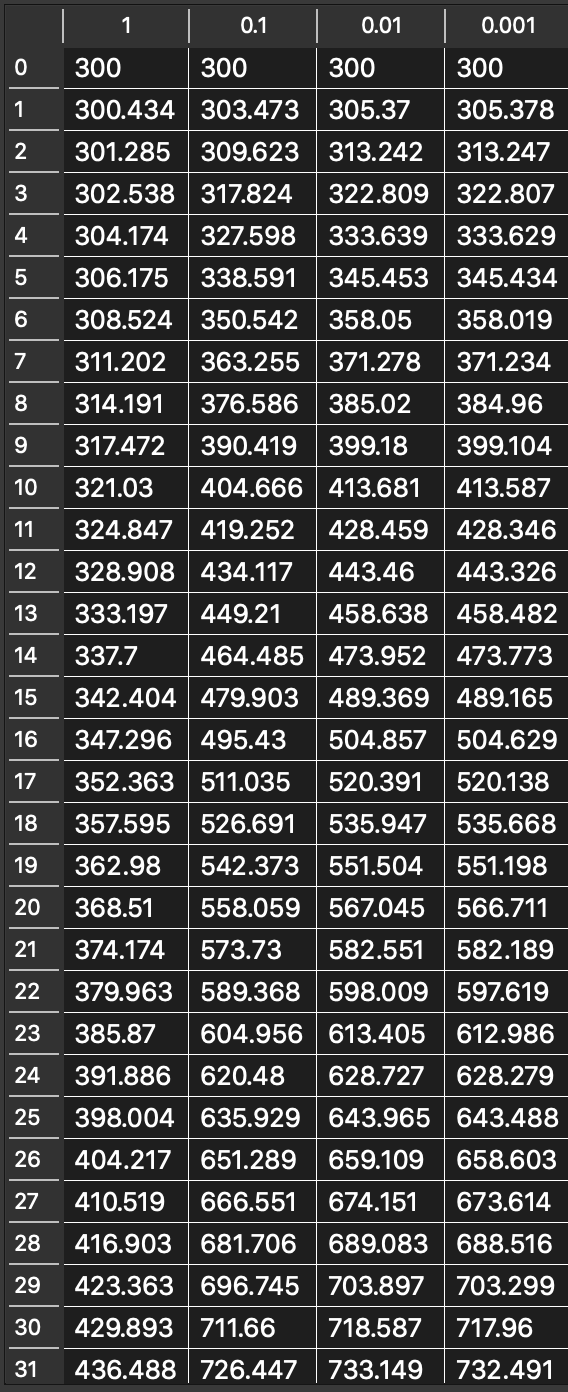
\includegraphics[scale=0.6]{img/steph.png}
            \caption{Шаг в пространстве}
            \label{img:steph}
        \end{figure}

        Рассматривая результаты, видимые на рисунке \ref{img:steph}, выбран оптимальный шаг $h = 0.01$.

        При выборе оптимального шага для времени необходимо рассмотреть результаты для разных $t_\text{max}$. На рисунке \ref{img:steptau10} рассмотрен случай при $t_\text{max} = 10$, а на \ref{img:steptau100} -- $t_\text{max} = 100$.

        \begin{minipage}{0.5\textwidth}
            \begin{flushleft}
                \begin{figure}[H]
                    \centering
                    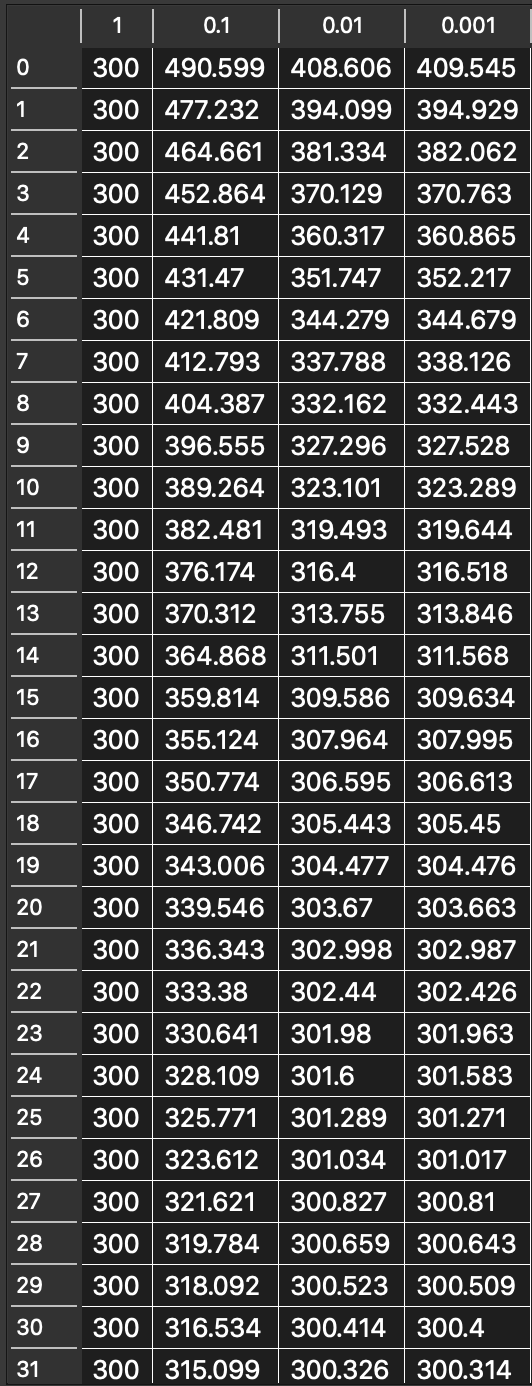
\includegraphics[scale=0.60]{img/steptau10.png}
                    \caption{Шаг по времени при $t_\text{max} = 10$}
                    \label{img:steptau10}
                \end{figure}
            \end{flushleft}
        \end{minipage}
        \begin{minipage}{0.5\textwidth}
            \begin{flushright}
                \begin{figure}[H]
                    \centering
                    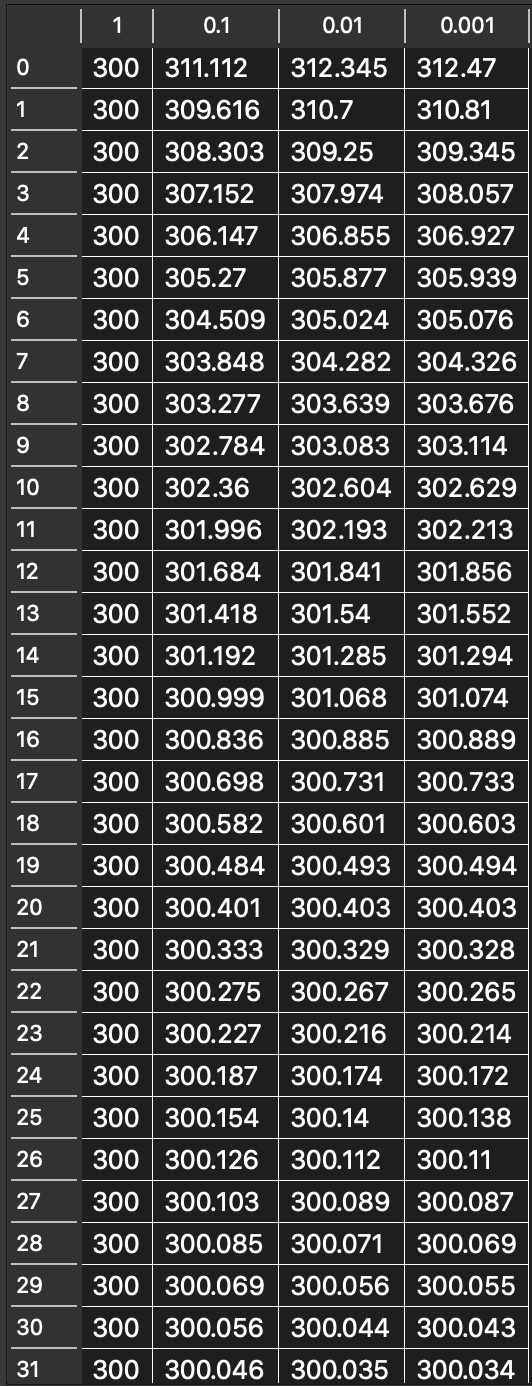
\includegraphics[scale=0.60]{img/steptau100.png}
                    \caption{Шаг по времени при $t_\text{max} = 100$}
                    \label{img:steptau100}
                \end{figure}
            \end{flushright}
        \end{minipage}

        При $t_\text{max} = 10$ оптимальный шаг $\tau = 0.01$, а при $t_\text{max} = 100$ -- $\tau = 0.1$. Таким образом, выбран оптимальный шаг $\tau = \frac{t_\text{max}}{1000}$.

        На рисунках \ref{img:xn100-10}, \ref{img:xn100-100}, \ref{img:xn500-100} видно влияние амплитуды импульса и времени достижения амплитуды.

        \begin{figure}[H]
            \centering
            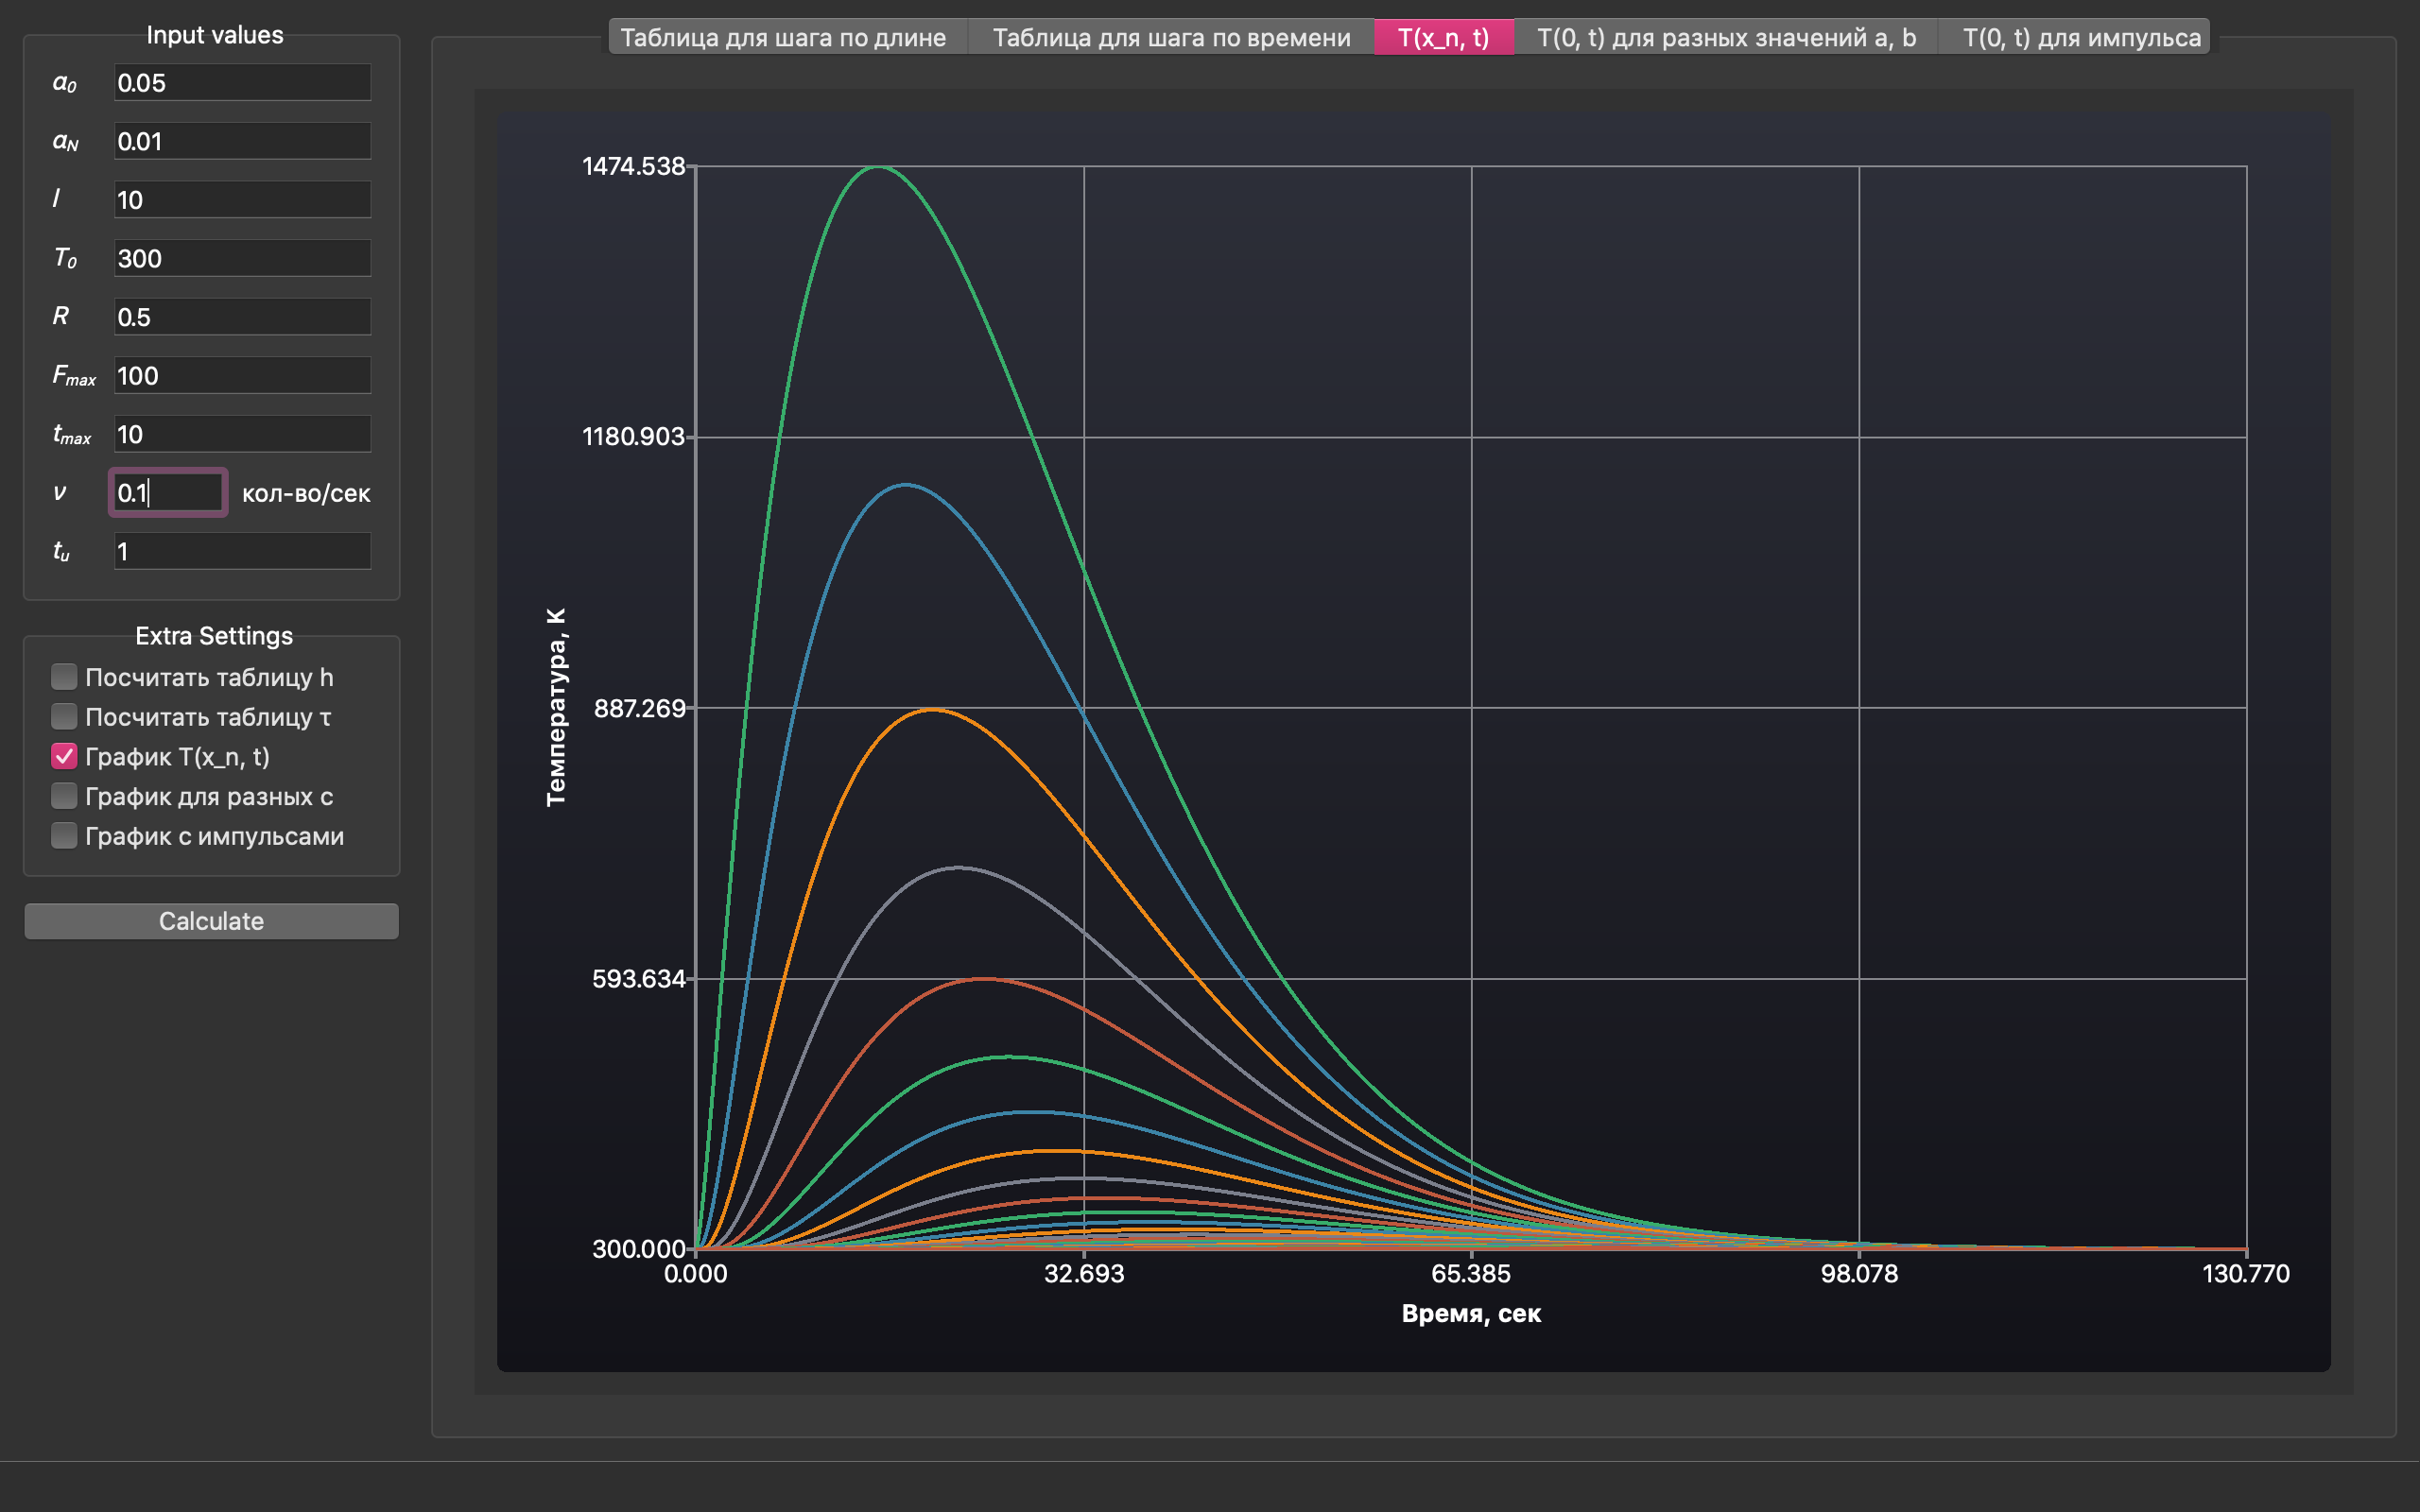
\includegraphics[scale=0.35]{img/xn100-10.png}
            \caption{График $T\big(x_n, t\big)$ при $F_\text{max} = 100,\ t_\text{max} = 10$}
            \label{img:xn100-10}
        \end{figure}

        \begin{figure}[H]
            \centering
            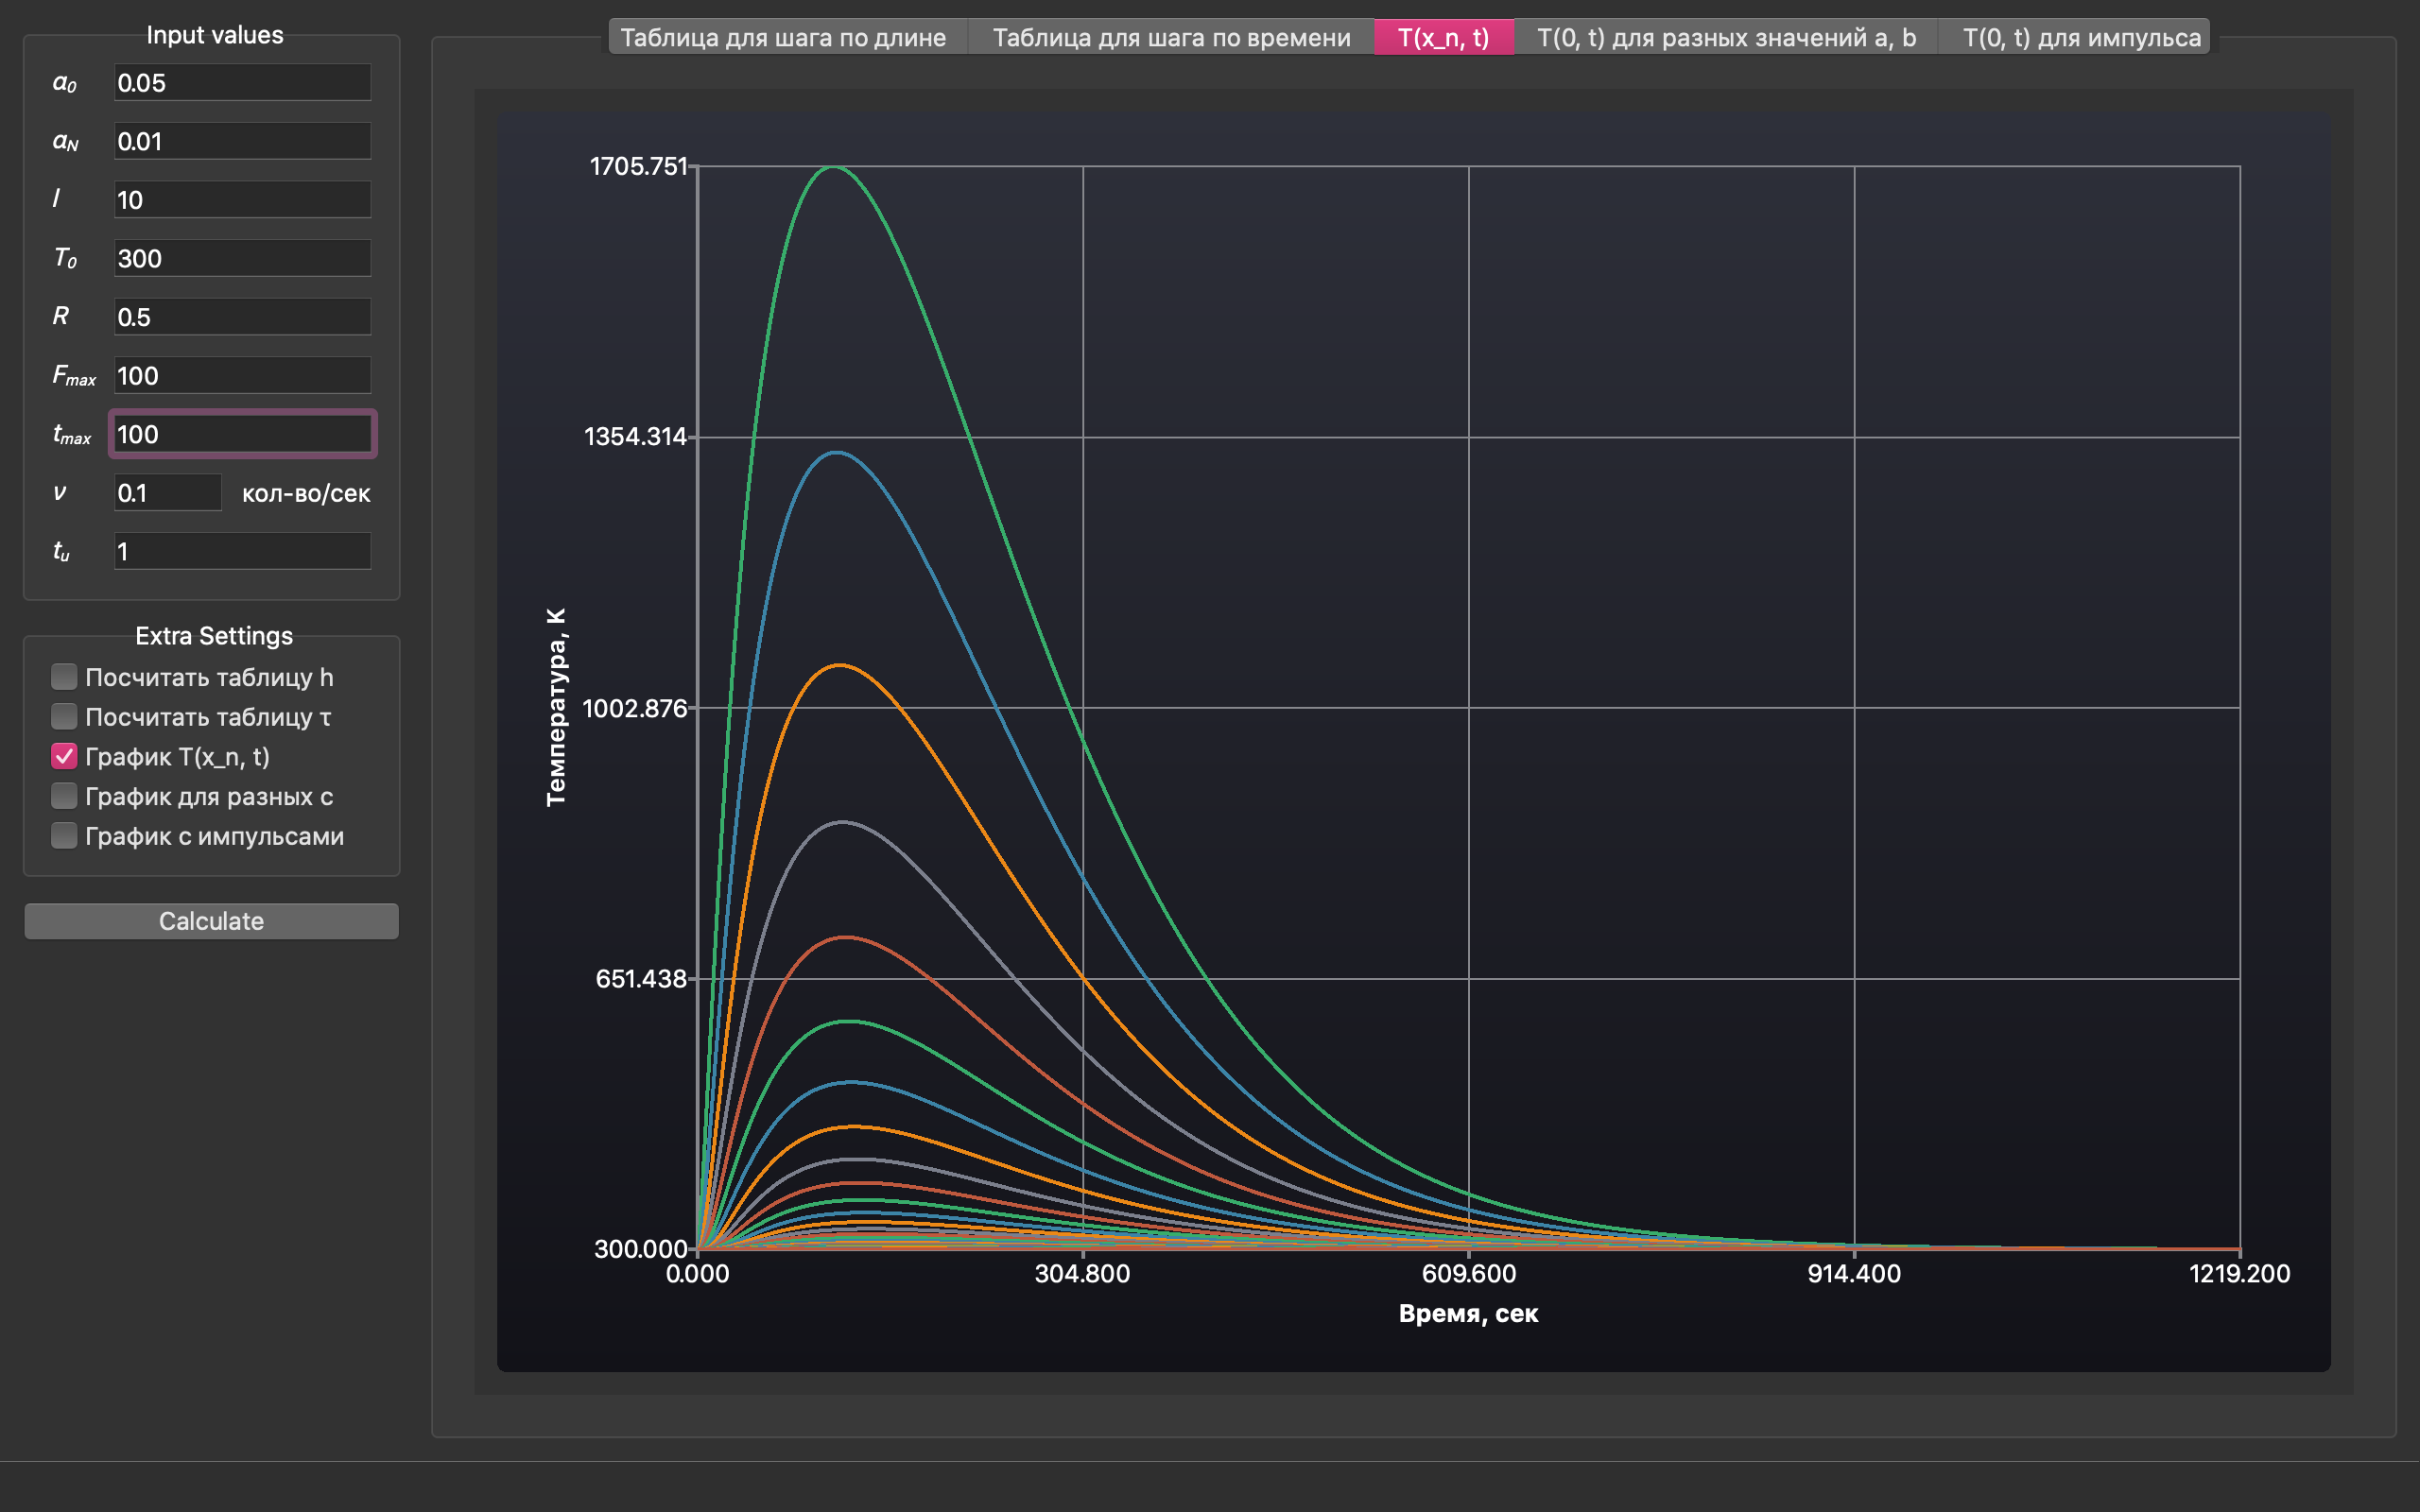
\includegraphics[scale=0.35]{img/xn100-100.png}
            \caption{График $T\big(x_n, t\big)$ при $F_\text{max} = 100,\ t_\text{max} = 100$}
            \label{img:xn100-100}
        \end{figure}

        \begin{figure}[H]
            \centering
            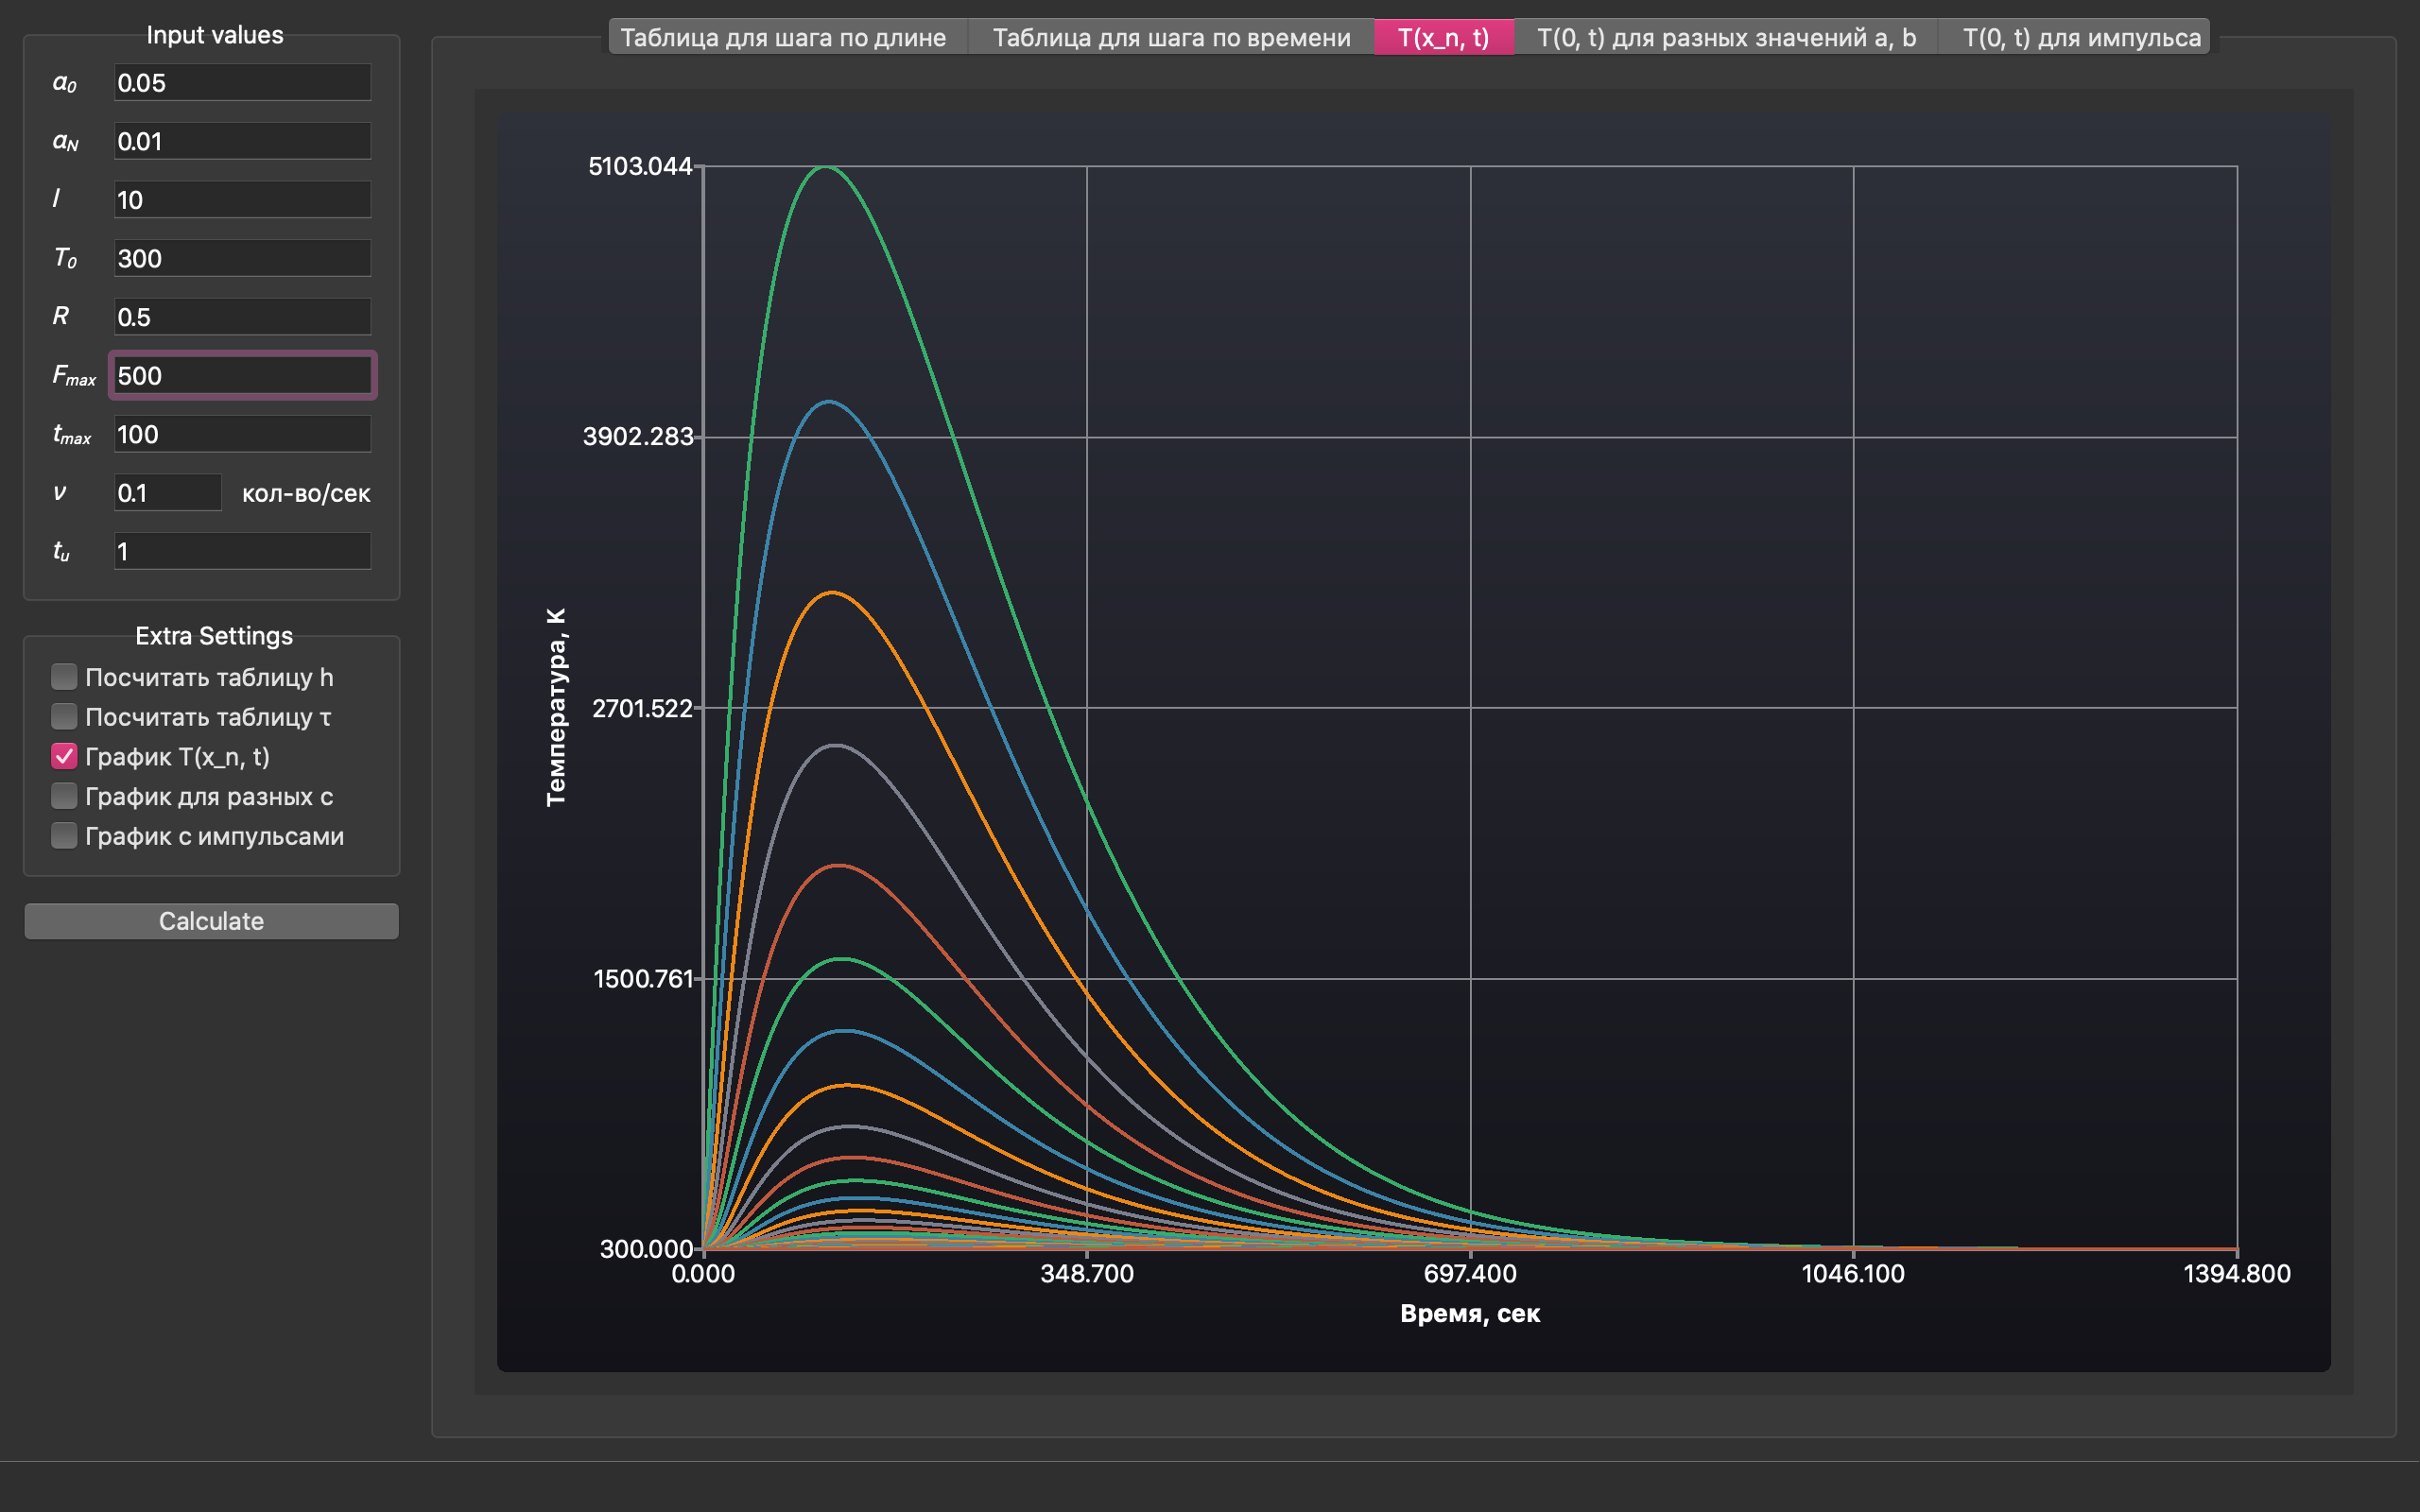
\includegraphics[scale=0.35]{img/xn500-100.png}
            \caption{График $T\big(x_n, t\big)$ при $F_\text{max} = 500,\ t_\text{max} = 100$}
            \label{img:xn500-100}
        \end{figure}

        Таким образом, можно заметить, что при увеличении $F_\text{max}$ возрастает максимальная температура стержня, а при изменении $t_\text{max}$ меняется время импульса и время достижения точки с максимальной температурой.

    \item \textbf{График зависимости температуры $T\big(0, t\big)$ при 3-4 значениях параметров $a_2$ и/или $b_2$ теплоемкости.}

        Параметры $a_2$ и $b_2$ принимают заданные значения из массивов, где для $a_2$ это {\ttfamily [2.049, 5, 10, 25]}, а для $b_2$ -- {\ttfamily [0.000564, 0.001, 0.01, 0.1]}. На рисунке \ref{img:capacity} видны графики для этих значений. Зеленый при $a_2 = 2.049$ и $b_2 = 564 \cdot 10^{-6}$, синий -- $a_2 = 5,\ b_2 = 0.001$, оранжевый -- $a_2 = 10\ b_2 = 0.01$ и серый -- $a_2 = 25,\ b_2 = 0.1$.

        \begin{figure}[H]
            \centering
            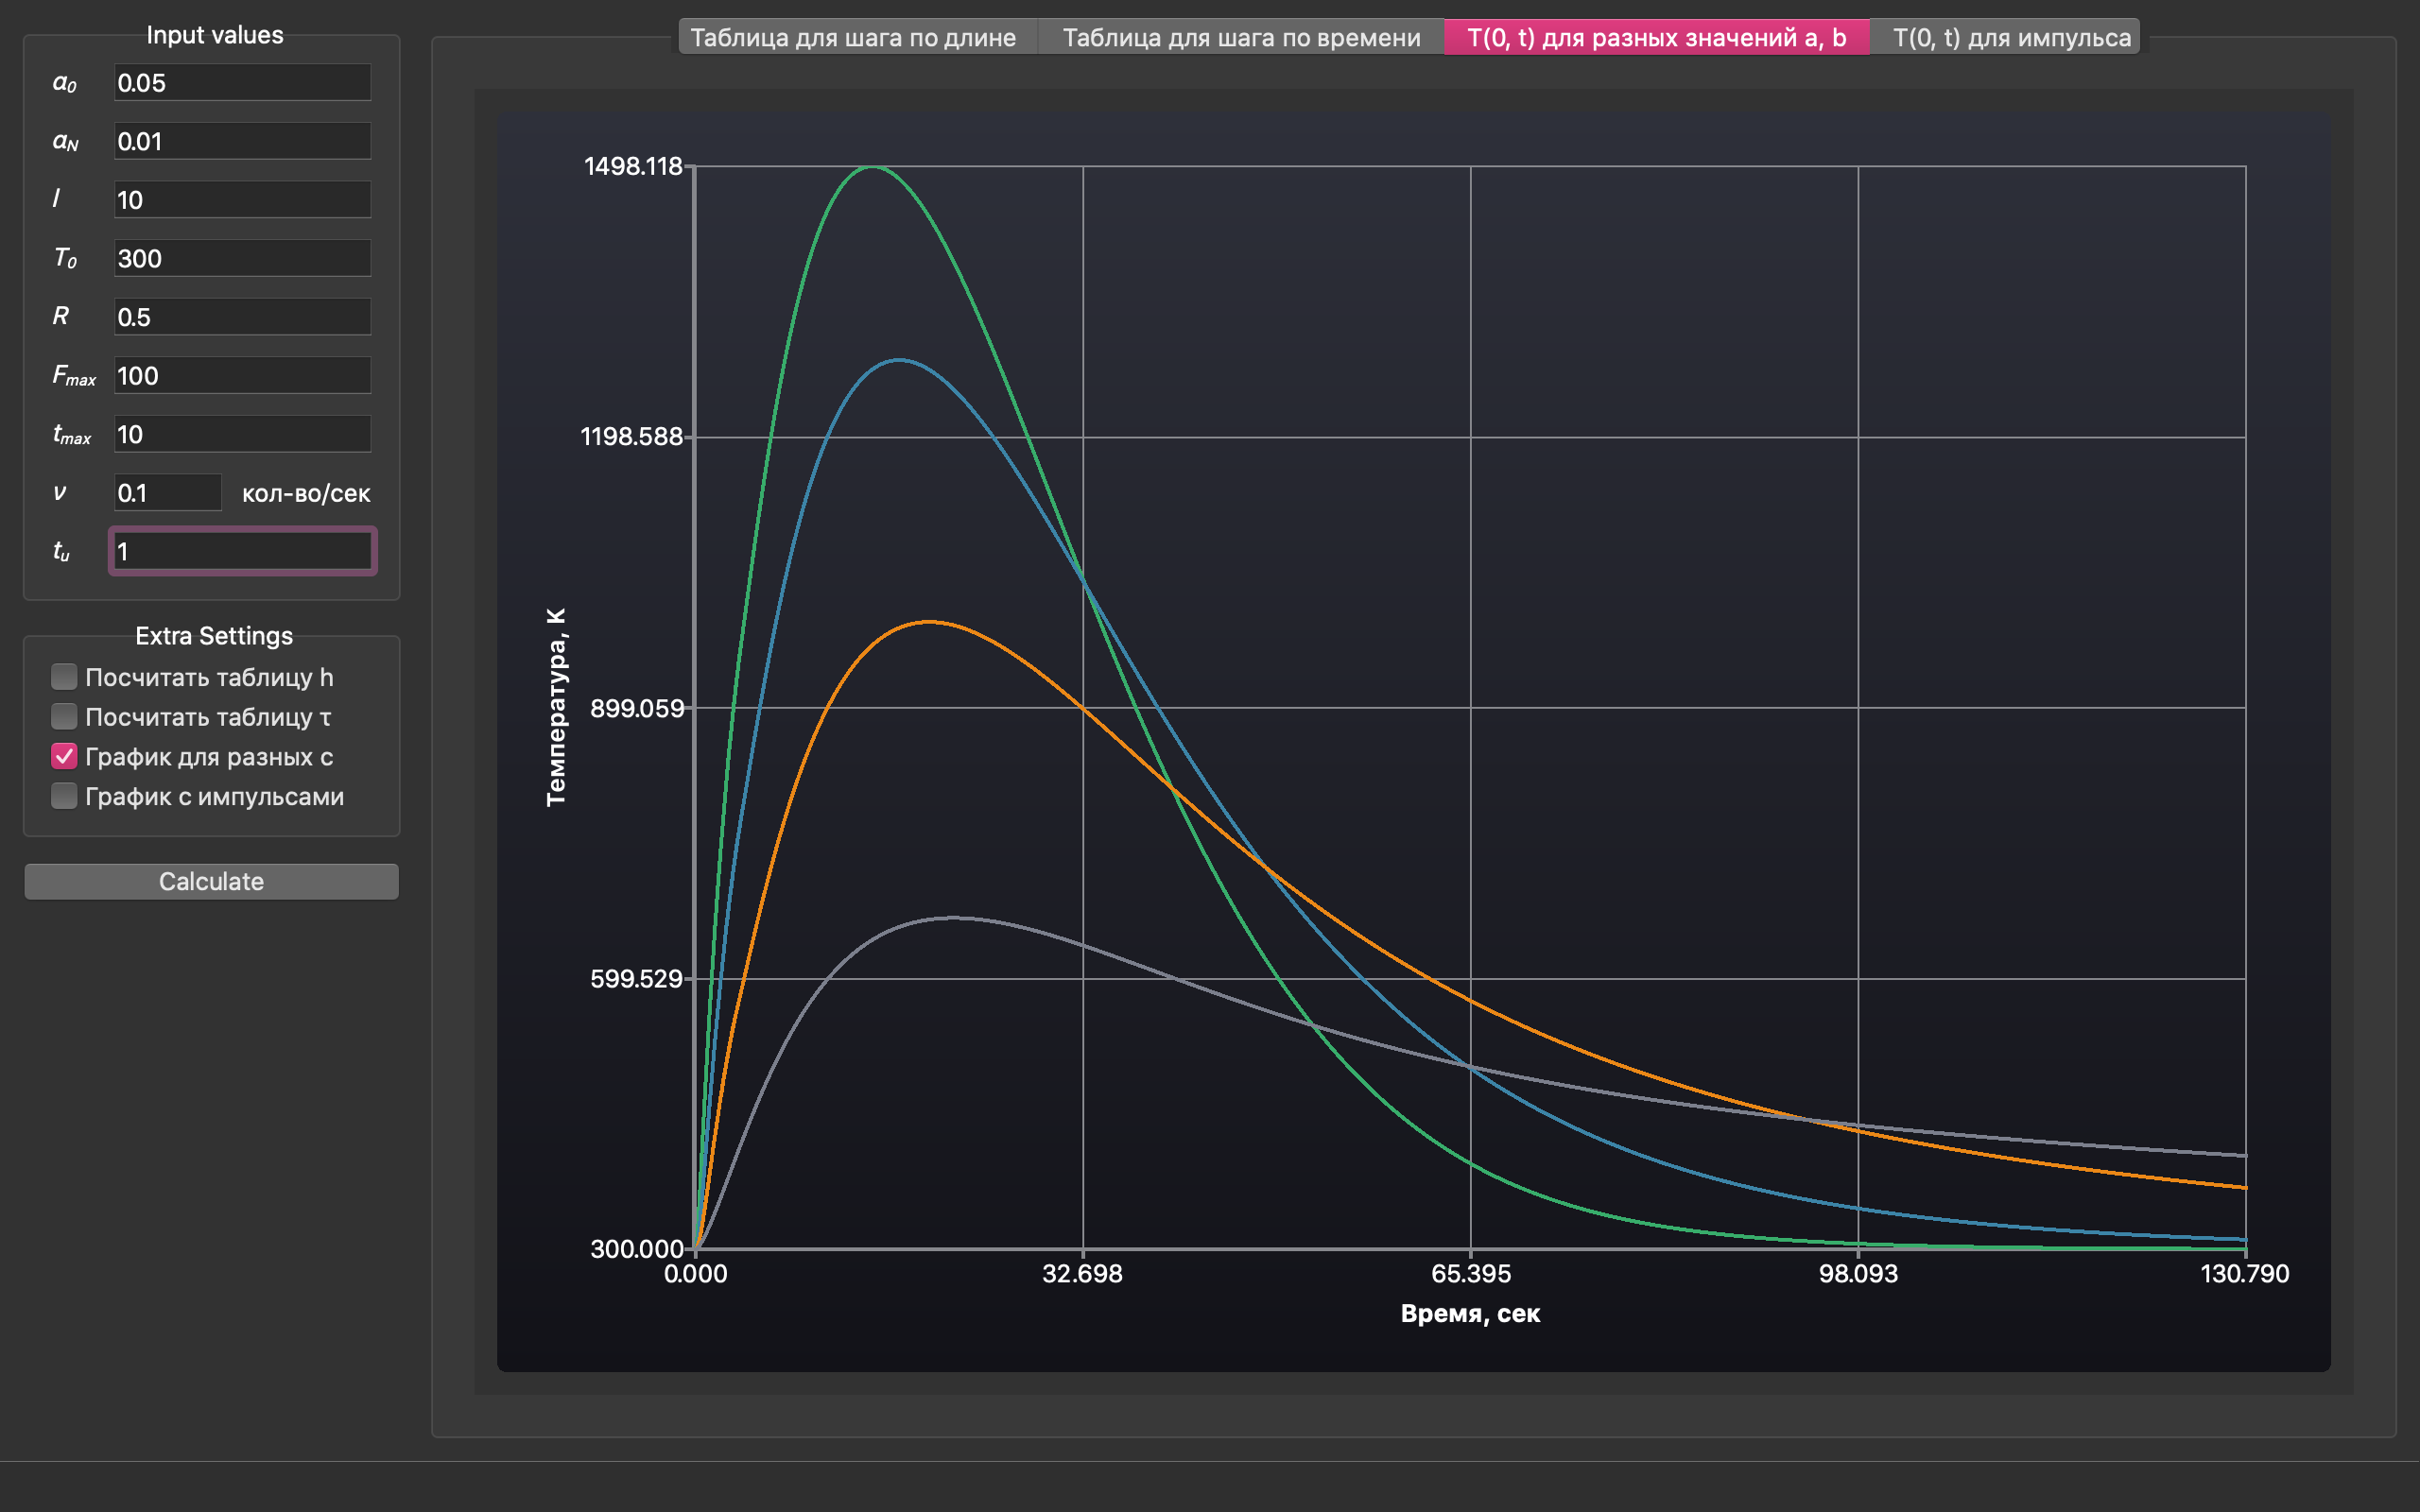
\includegraphics[scale=0.35]{img/capacity.png}
            \caption{График $T\big(0, t \big)$ при разных значениях $a_2$, $b_2$}
            \label{img:capacity}
        \end{figure}

        По этим графикам можно сделать вывод, что с увеличением теплоемкости темп роста и максимально значение температуры уменьшаются.

    \item \textbf{График зависимости температуры $T\big( 0, t \big)$ (т.е. при $x = 0$ ) в частотном режиме теплового нагружения. Импульсы следуют один за другим с заданной частотой $\nu$ (частота определяется количеством импульсов в 1 секунду).}

        Подобраны такие $F_\text{max}$ и $t_\text{max}$, чтобы температуры не выходила за пределы 2000 K. На рисунках \ref{img:impulse1}, \ref{img:impulse2}, \ref{img:impulse3}, \ref{img:impulse4} видно, что при увеличении частоты размах колебаний температуры уменьшается вплоть до нуля, как видно на рисунке \ref{img:impulse4}.

        \begin{figure}[H]
            \centering
            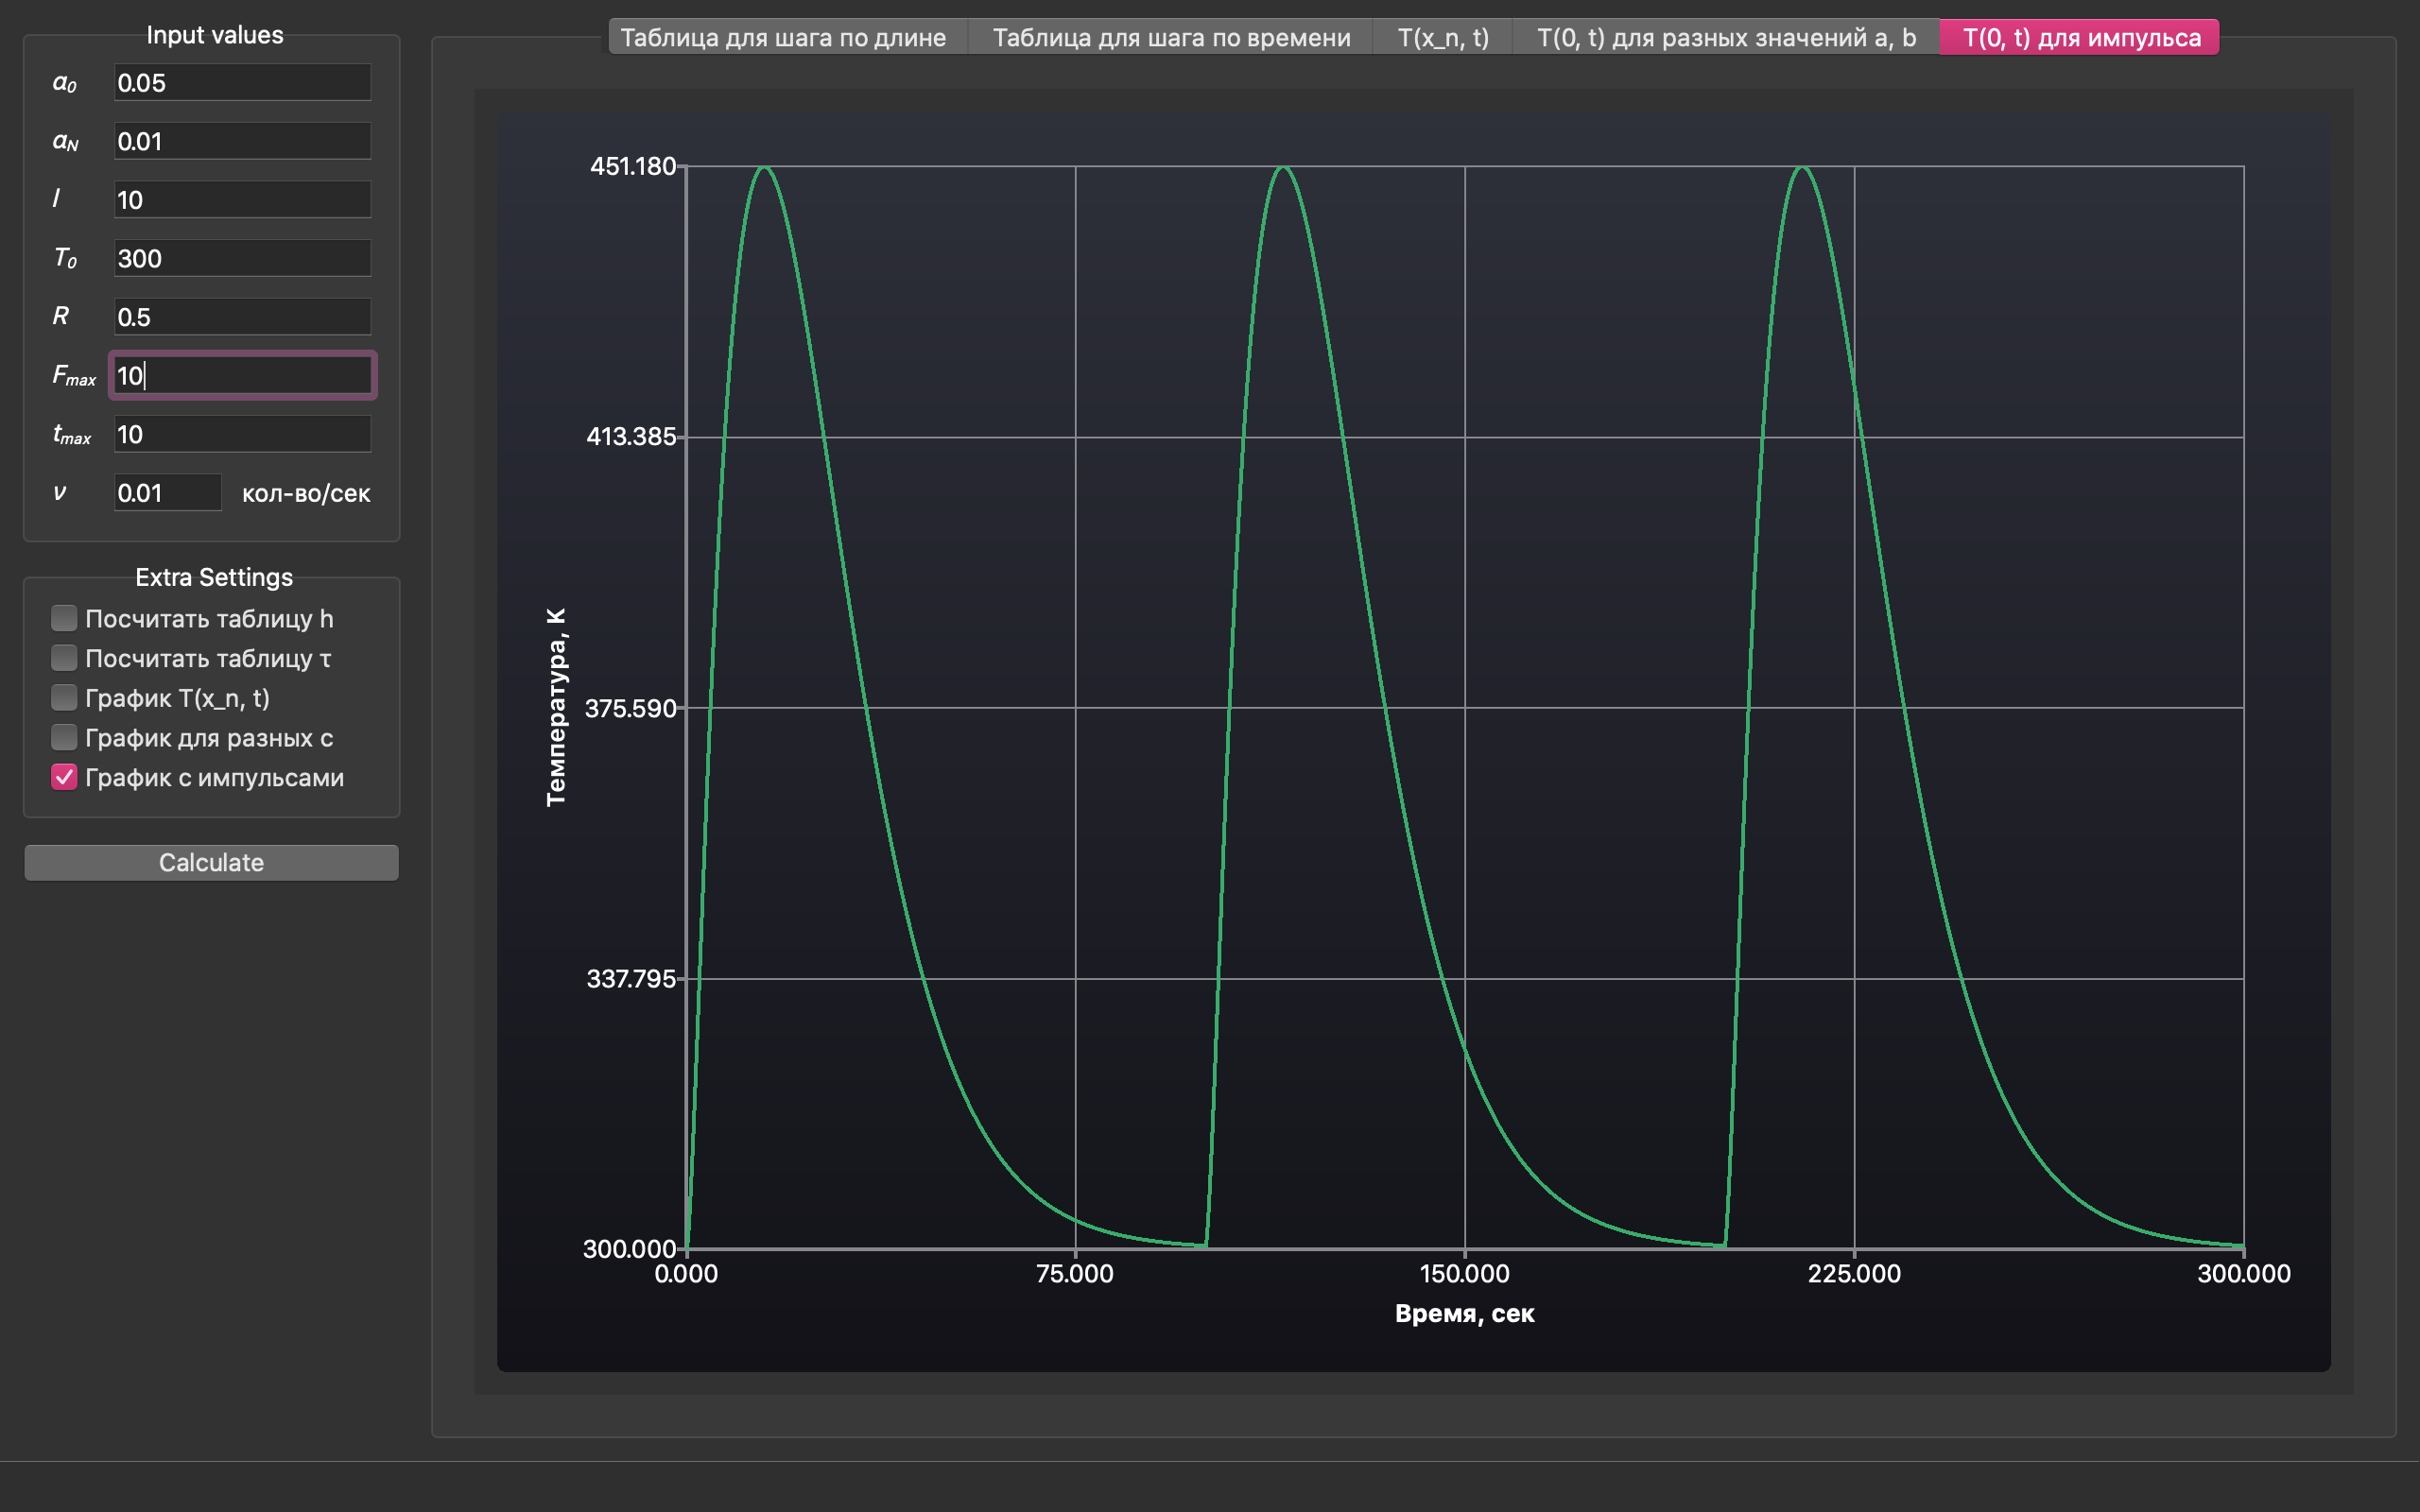
\includegraphics[scale=0.35]{img/impulse1.png}
            \caption{Частота $\nu = 0.01$}
            \label{img:impulse1}
        \end{figure}

        \begin{figure}[H]
            \centering
            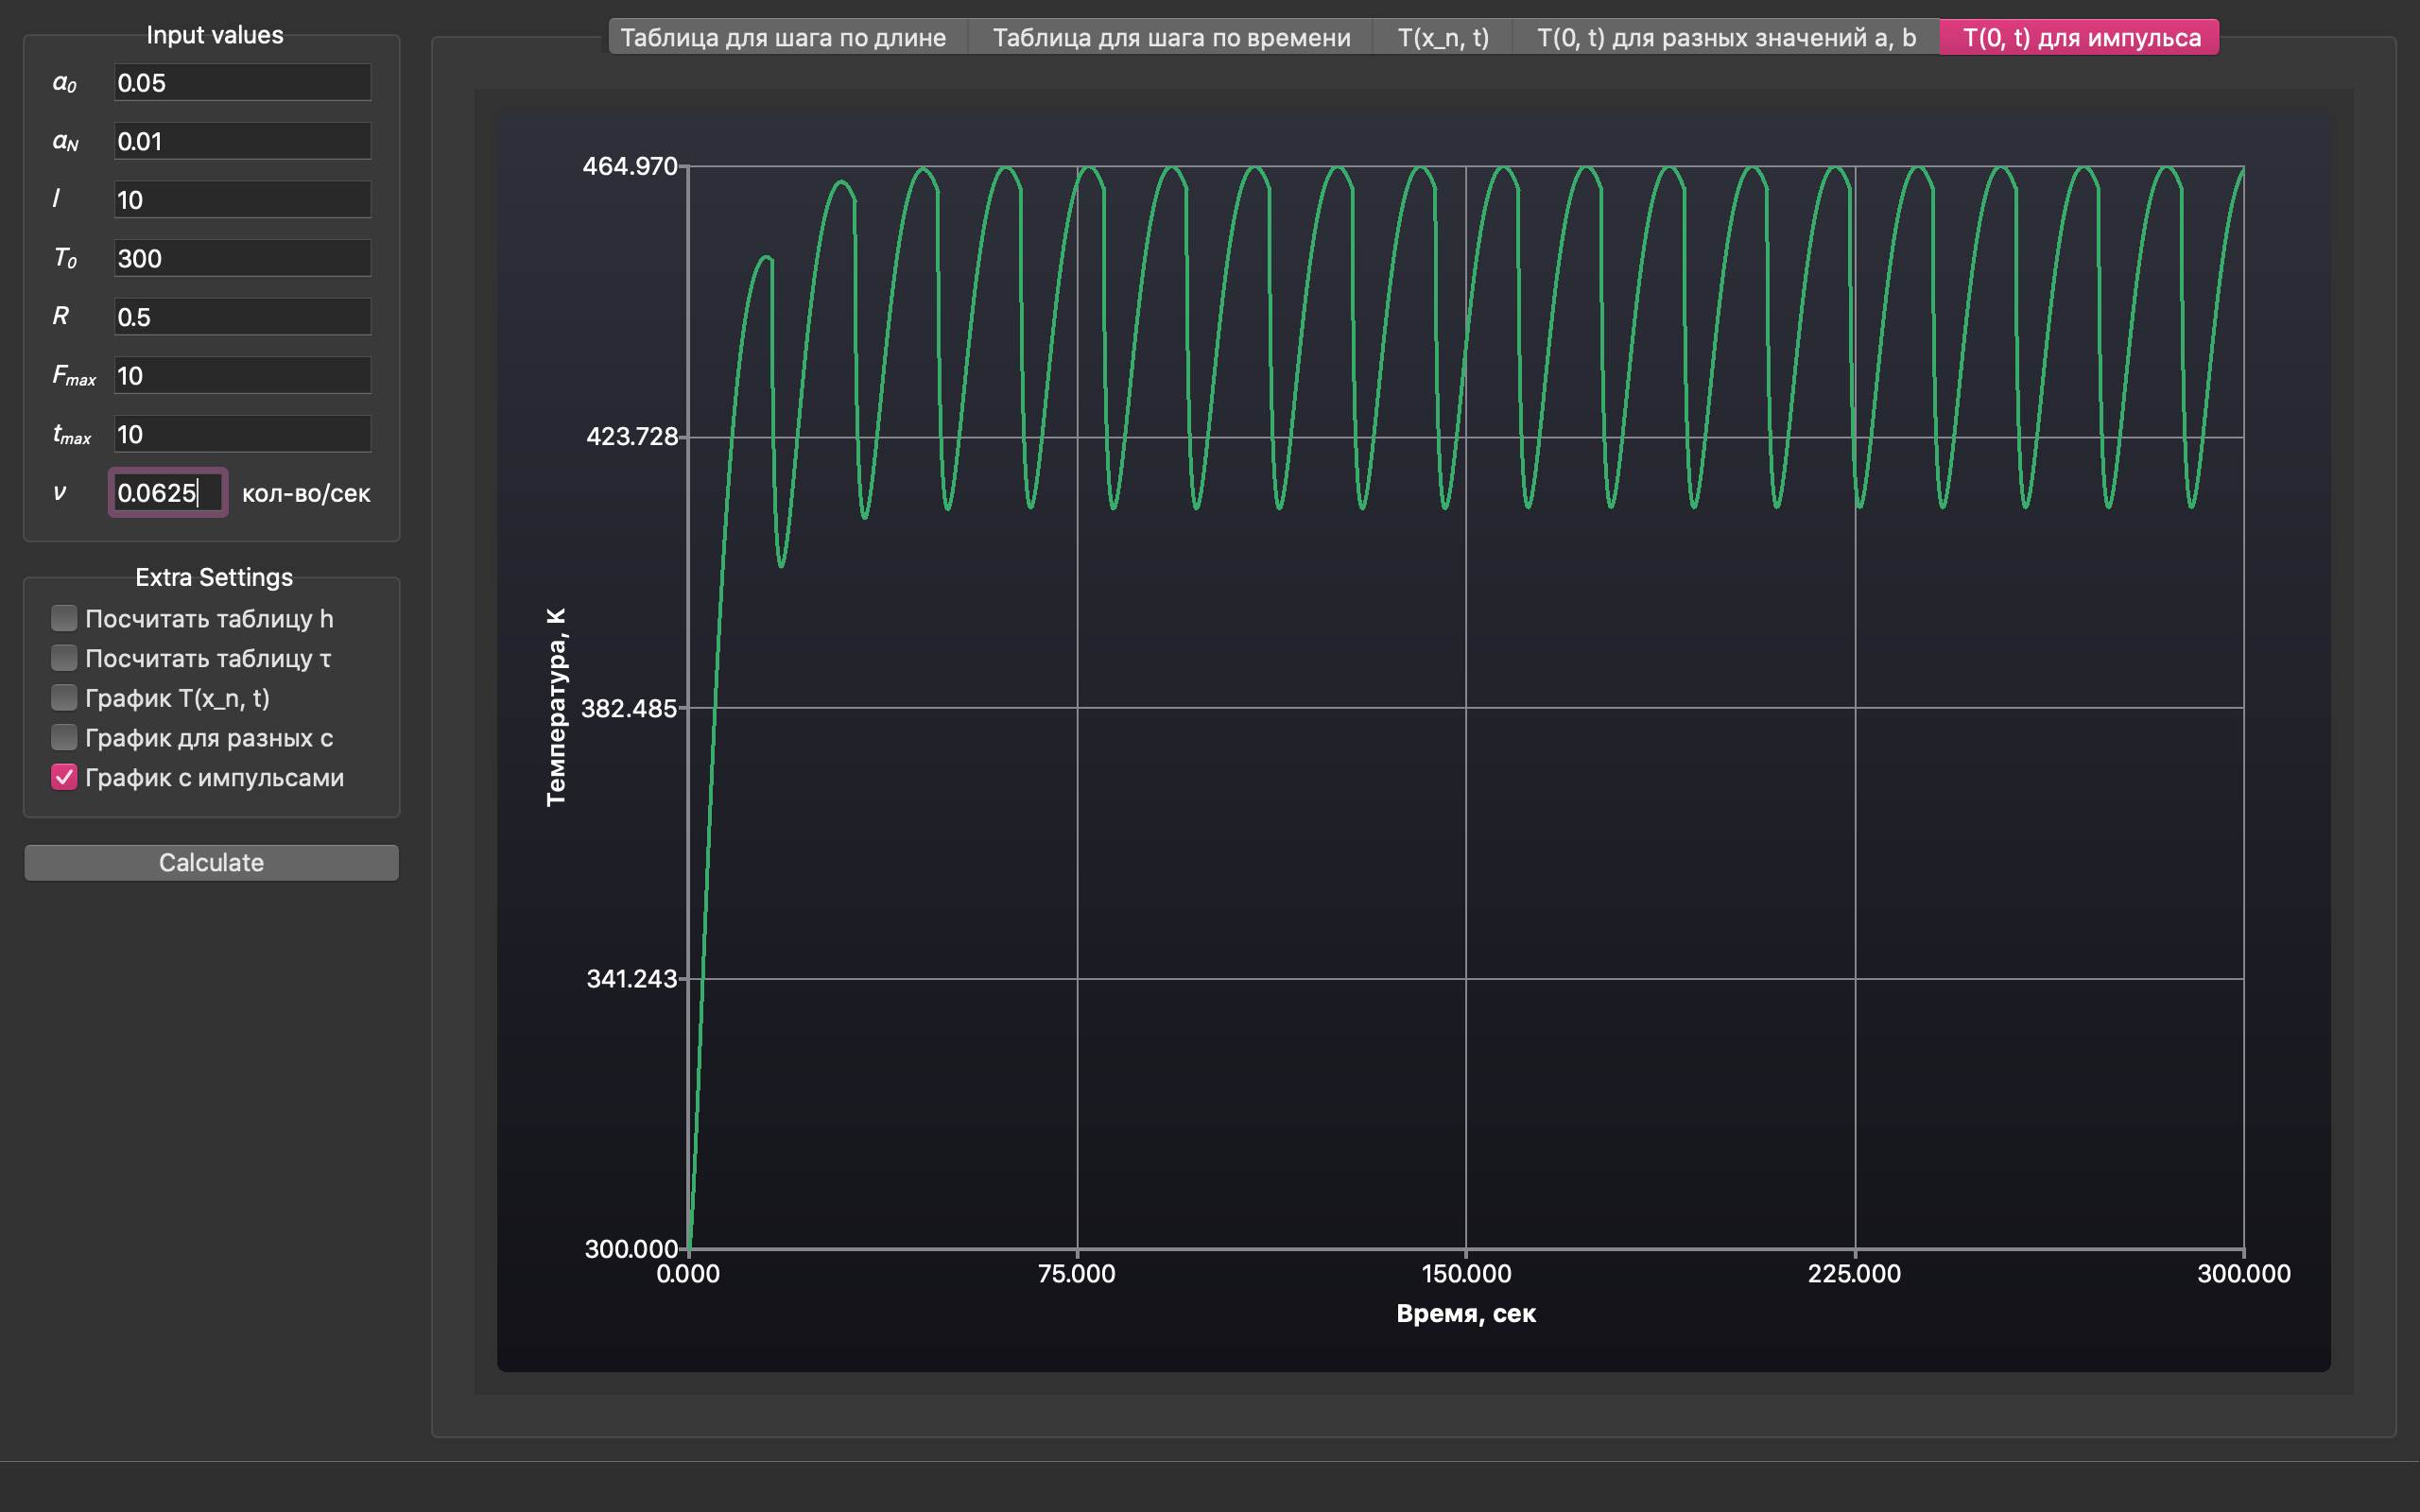
\includegraphics[scale=0.35]{img/impulse2.png}
            \caption{Частота $\nu = 0.0625$}
            \label{img:impulse2}
        \end{figure}

        \begin{figure}[H]
            \centering
            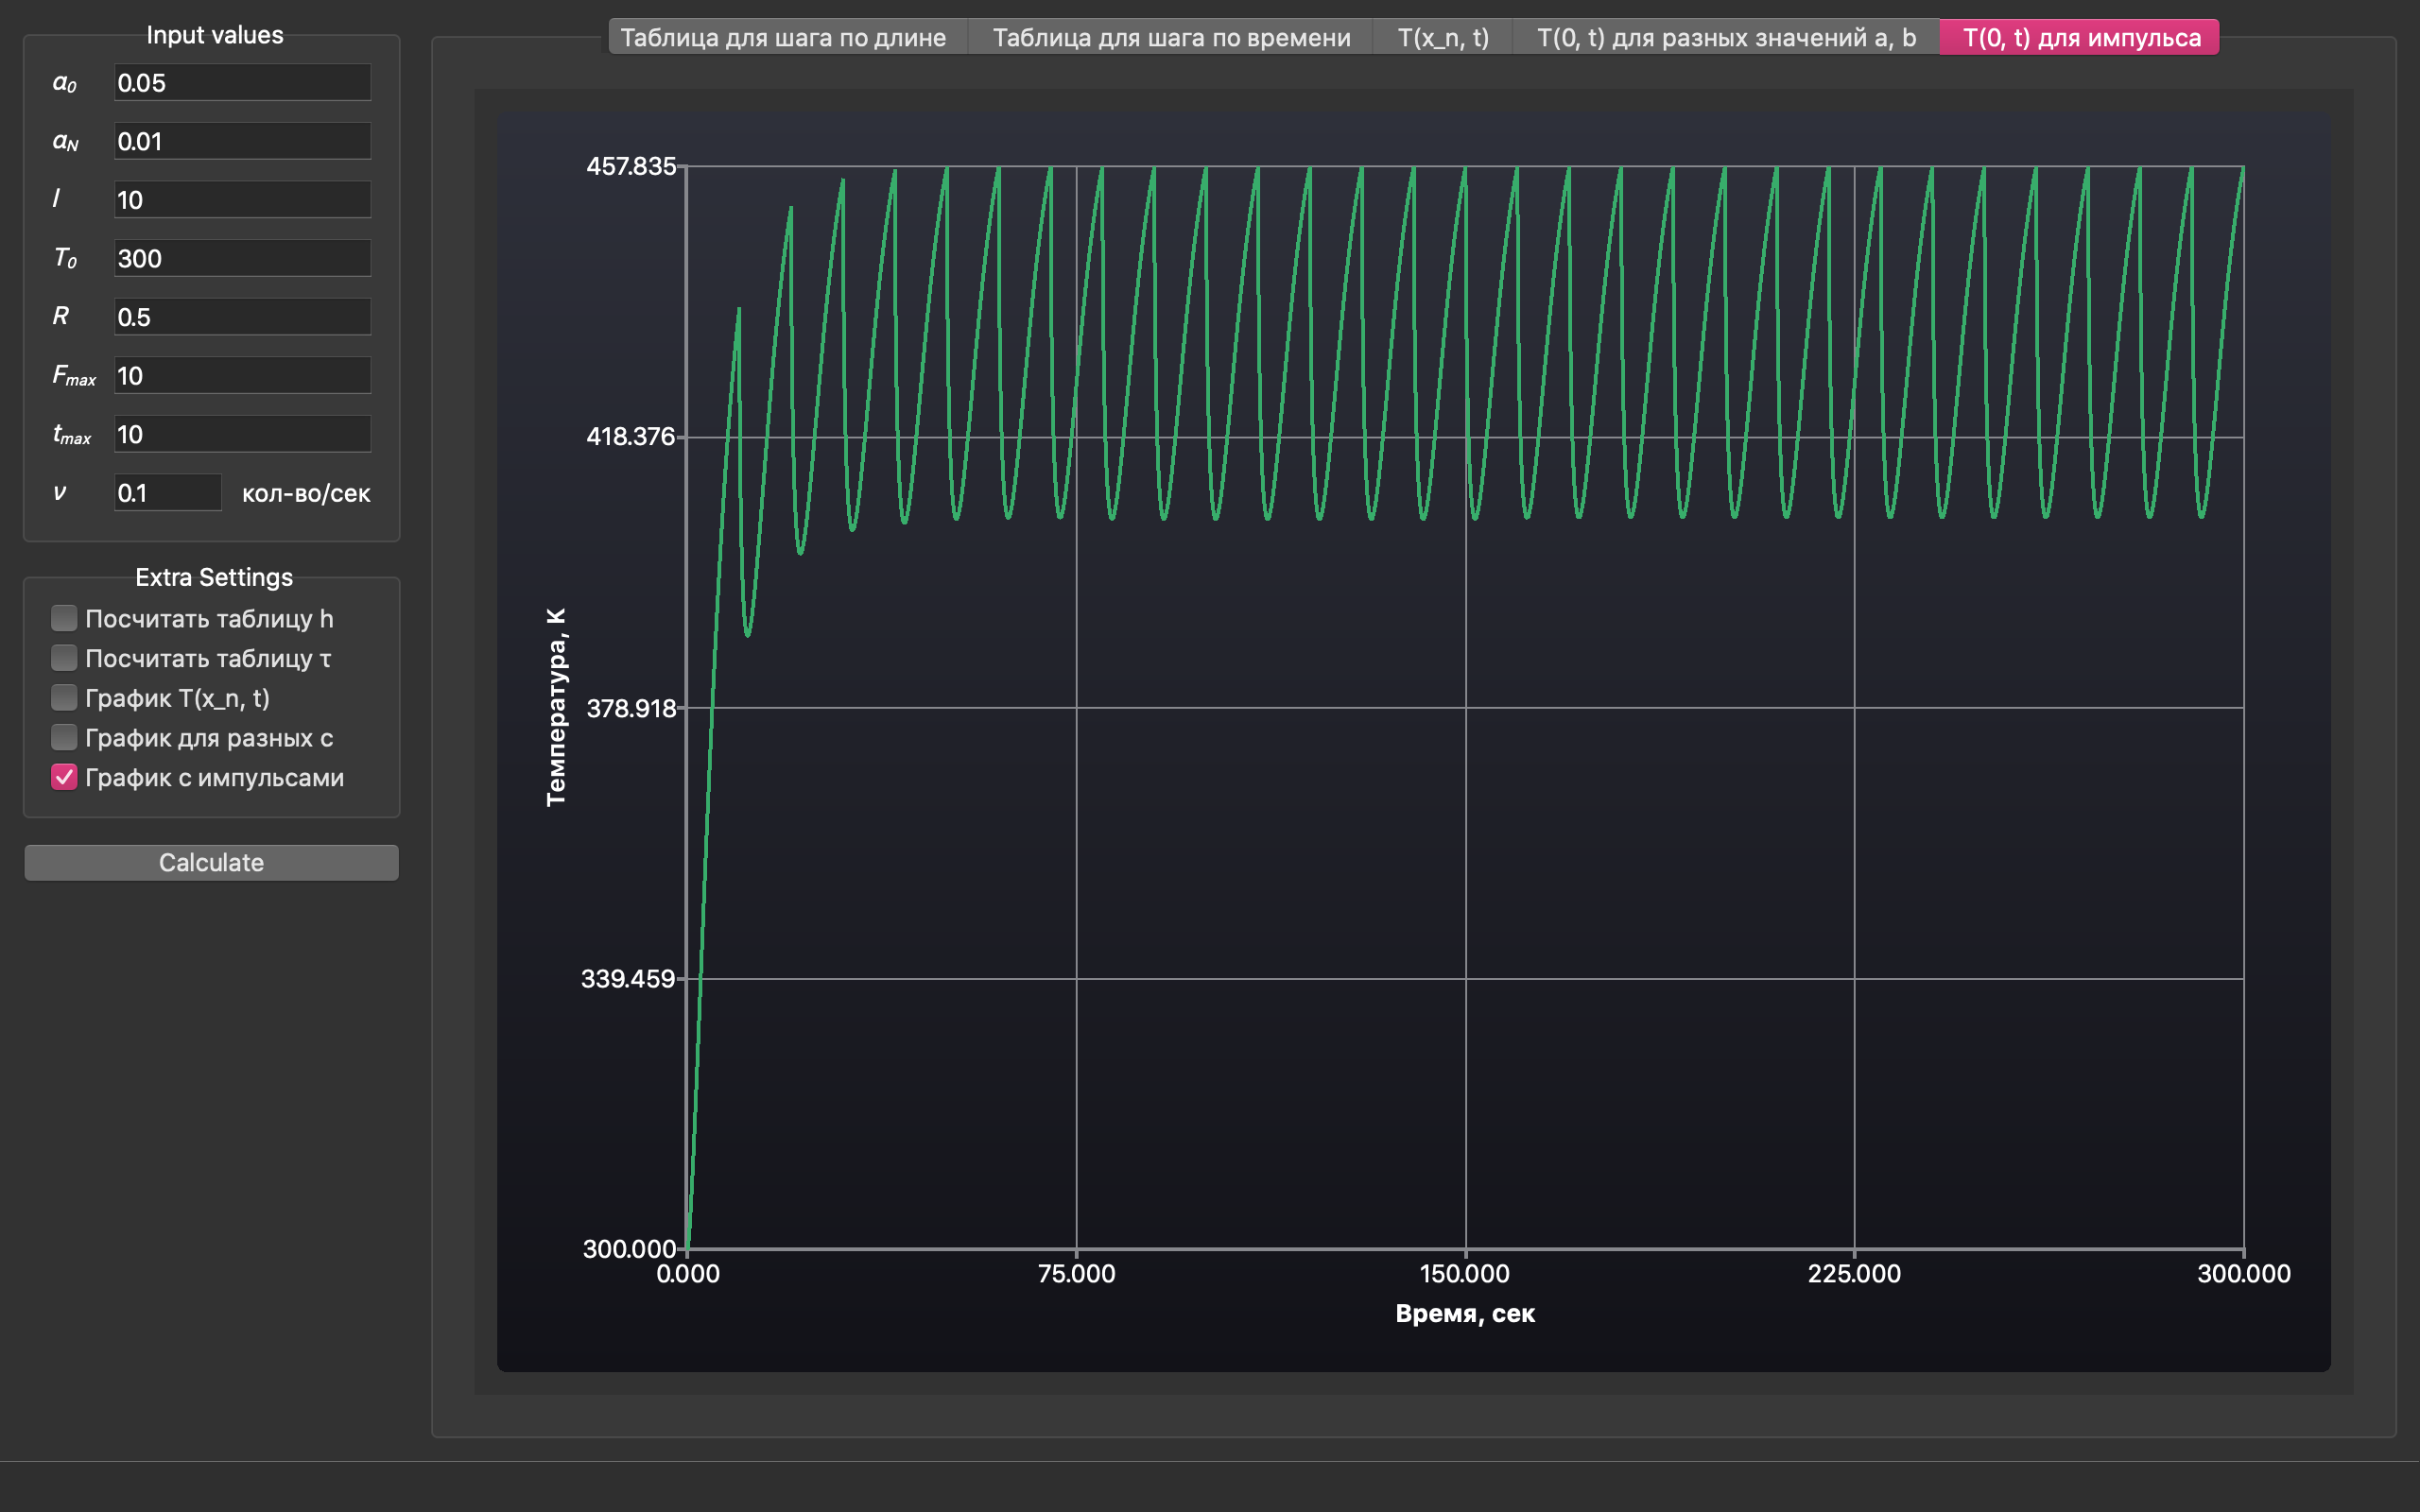
\includegraphics[scale=0.35]{img/impulse3.png}
            \caption{Частота $\nu = 0.1$}
            \label{img:impulse3}
        \end{figure}

        \begin{figure}[H]
            \centering
            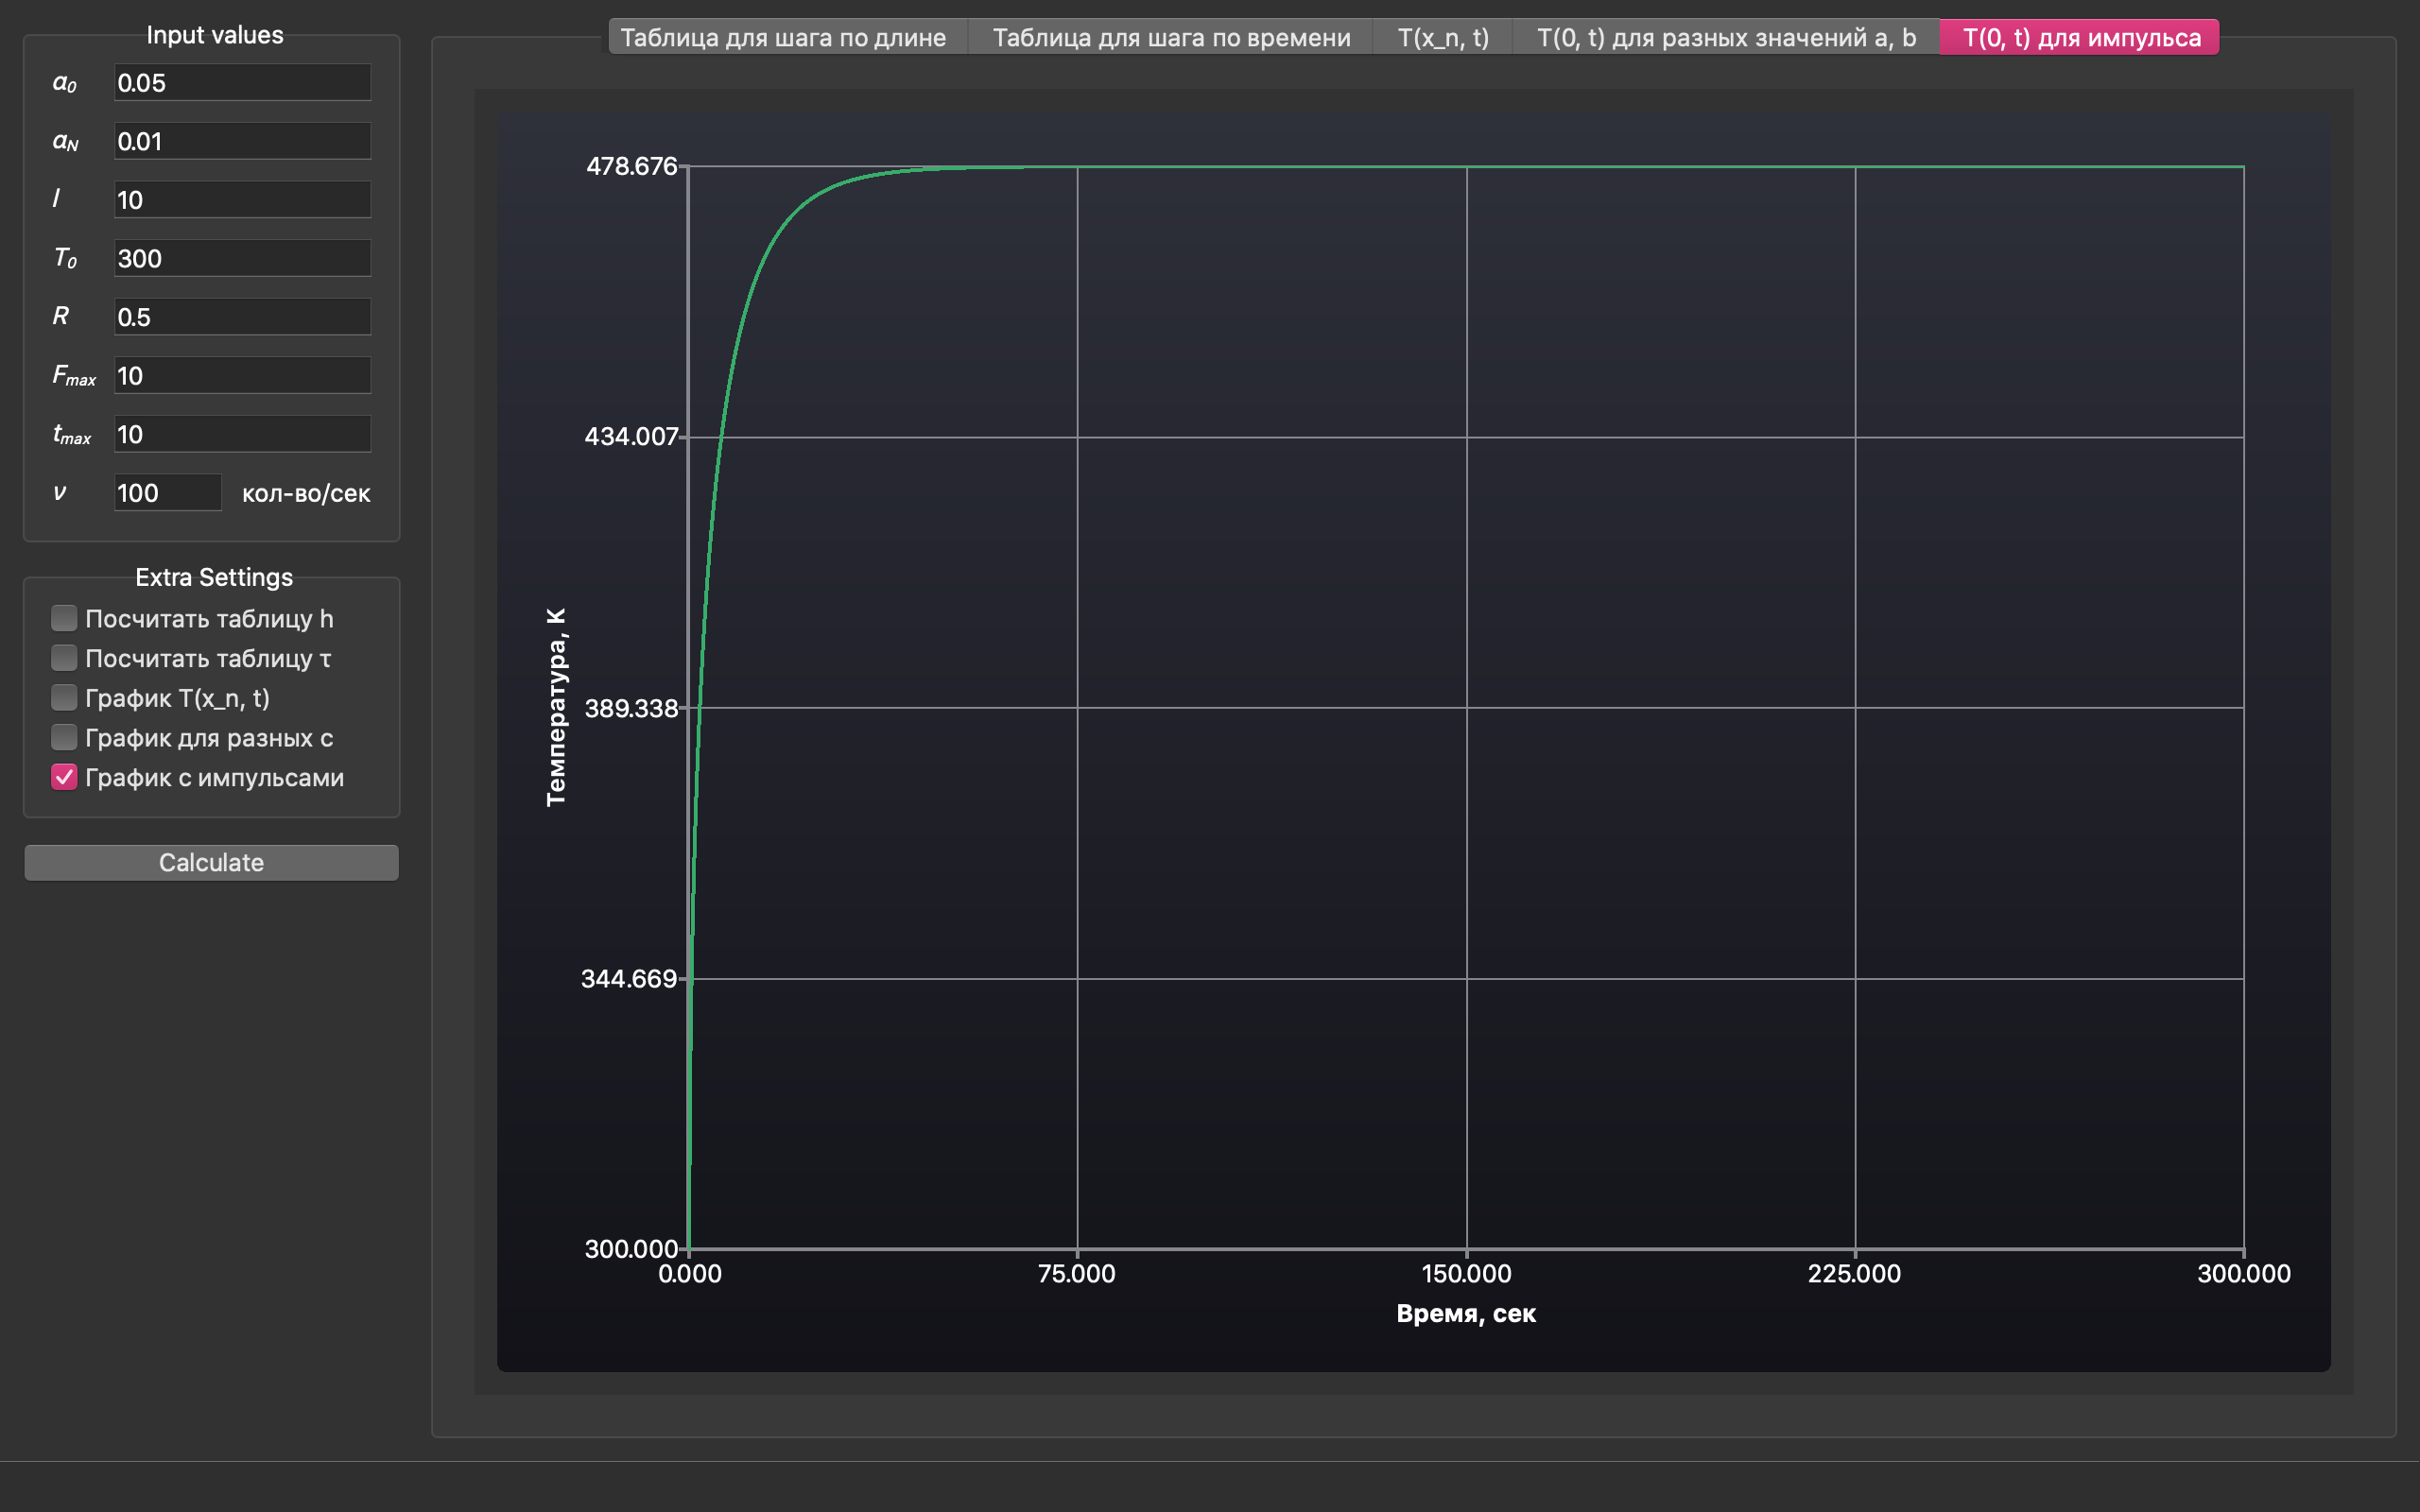
\includegraphics[scale=0.35]{img/impulse4.png}
            \caption{Частота $\nu = 100$}
            \label{img:impulse4}
        \end{figure}

        Полученное температурное поле совпадает с результатом расчета по программе лабораторной работы №3 при всех одинаковых параметрах модели. На рисунке \ref{img:lab_03} график, полученный программой из третьей лабораторной работы, а на рисунке \ref{img:lab_03_new} -- из текущей.

        \begin{figure}[H]
            \centering
            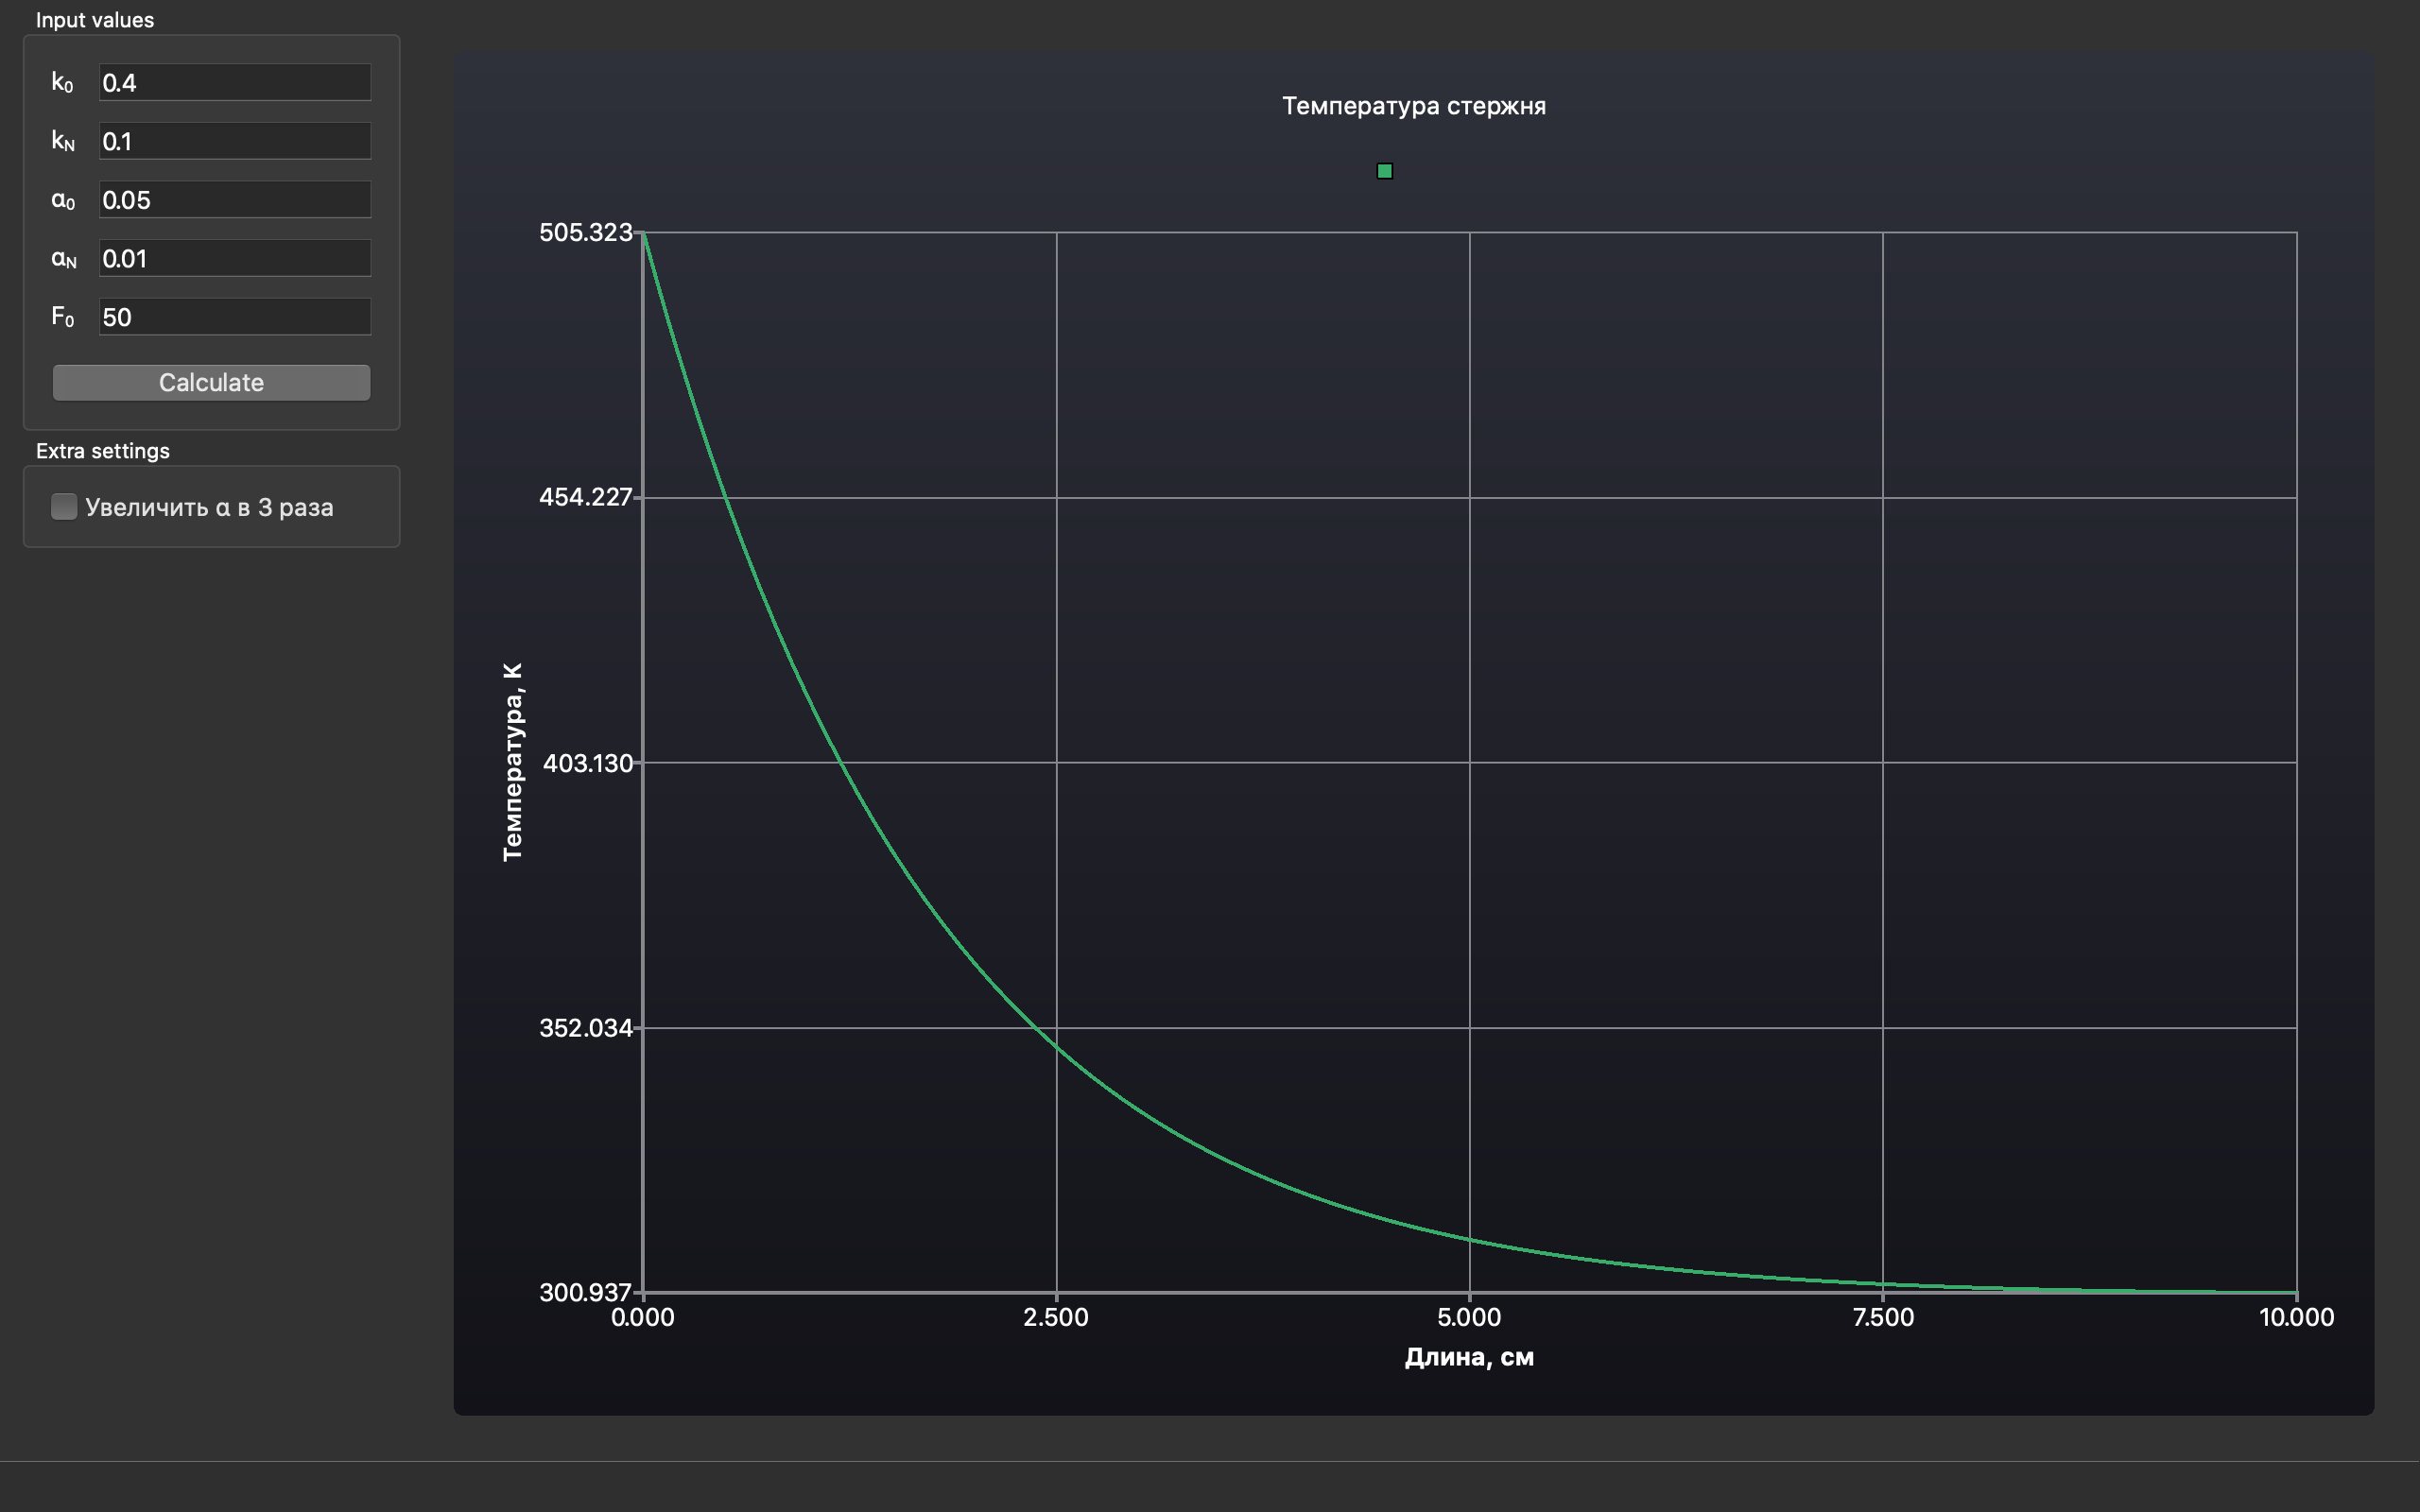
\includegraphics[scale=0.35]{img/lab_03.png}
            \caption{График из третьей лабораторной работы}
            \label{img:lab_03}
        \end{figure}

        \begin{figure}[H]
            \centering
            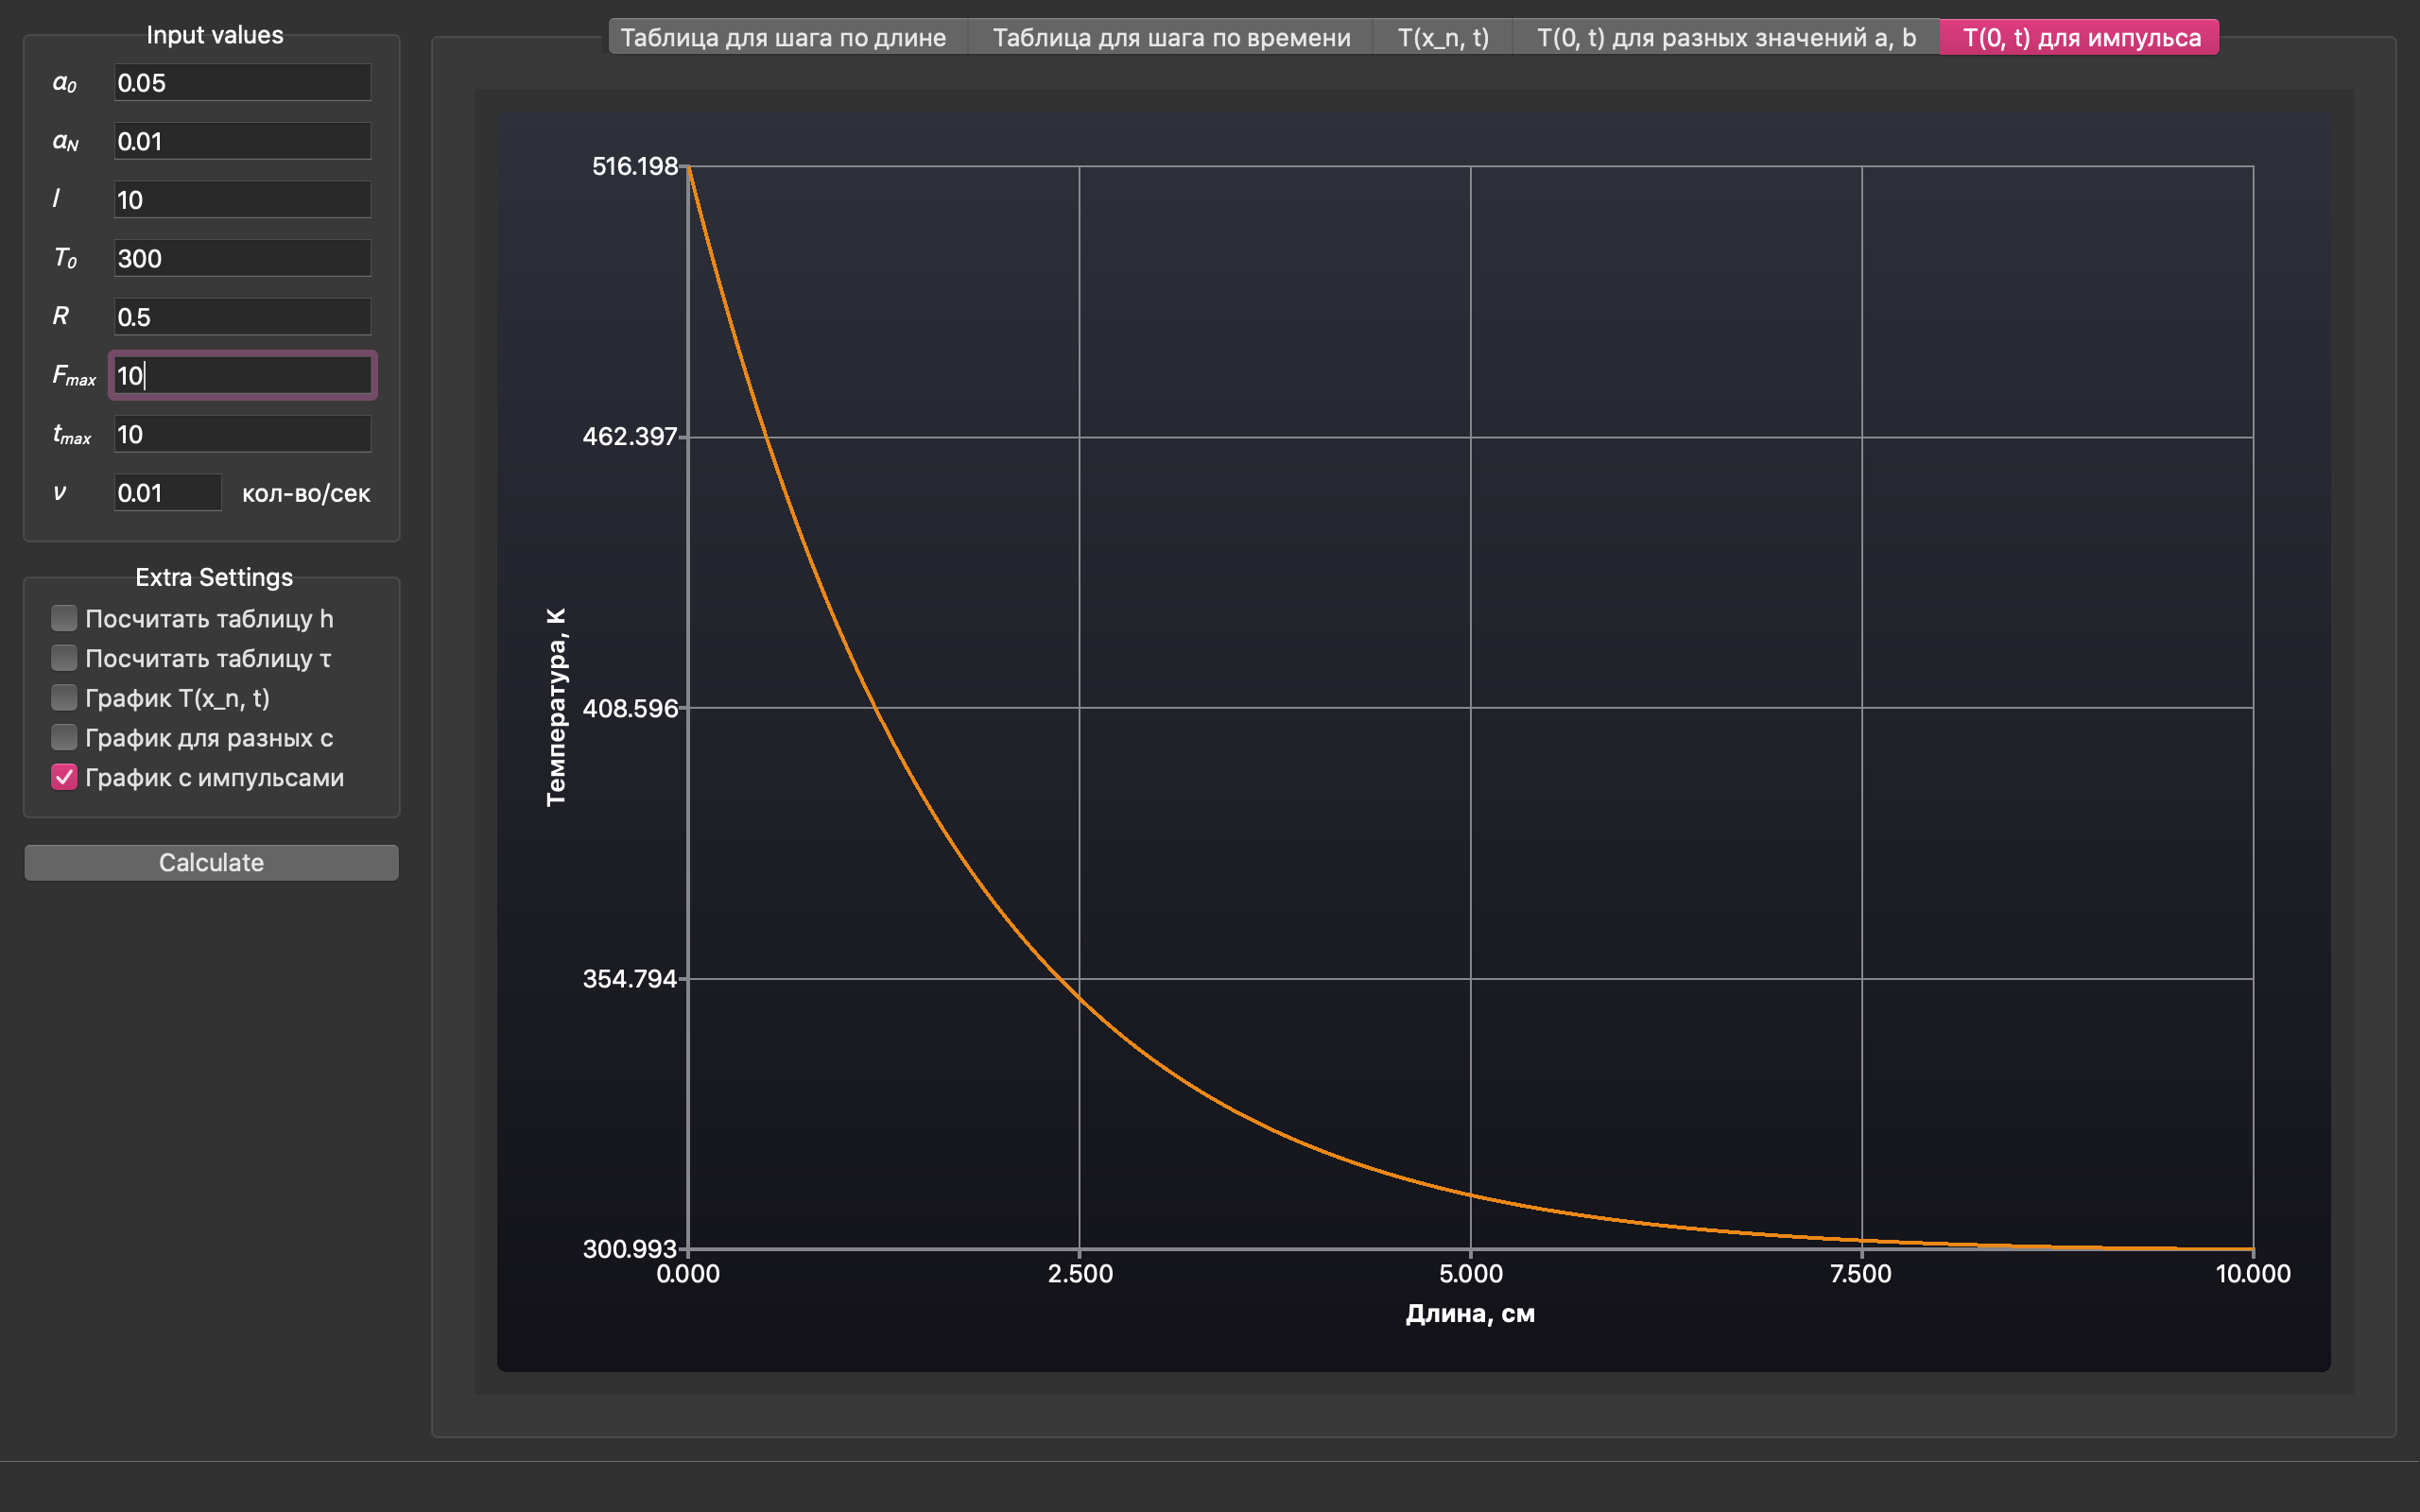
\includegraphics[scale=0.35]{img/lab_03_new.png}
            \caption{График из текущей лабораторной работы}
            \label{img:lab_03_new}
        \end{figure}
\end{enumerate}
